\chapter{Sistema de carga multiquímica}

Para la carga de la batería Li-ion se escogió el método de carga CC/VC
descrito en la sección \ref{sec:alg_lion}, la máxima corriente de carga
se estableció en $1\text{A}$. Para la carga de la batería NiMH se utilizó
el método de \textit{trikle charge} descrito en la sección 
\ref{sec:alg_nimh}. Se empleó el mismo convertidor reductor para la carga
de ambas baterías, por lo que no es posible cargar ambas al mismo tiempo, esto
debido al espacio reducido del que se dispone para la colocación de componentes
en el PCB.
Para determinar que batería será cargada se utilizó un multiplexor de potencia
construido con transistores MOSFET de canal P.
    

    
\section{Convertidor reductor}
    \label{sec:buck_design}

    El sistema de carga multiquímica debe ser capaz de  proporcionar una 
    corriente constante para la carga de ambos tipos de baterías. Para ello
    se decidió emplear un convertidor reductor, el cual tiene por componente principal
    el circuito integrado LM2596. Para poder realizar un control del voltaje de salida ( y de
    forma indirecta la corriente del mismo)
    de forma electrónica, es decir aplicando un voltaje, se realizó una modificación al circuito
    de realimentación del circuito como es mostrado en la figura \ref{fig:buck_modificado}.

    \begin{figure}[H]
        \centering
        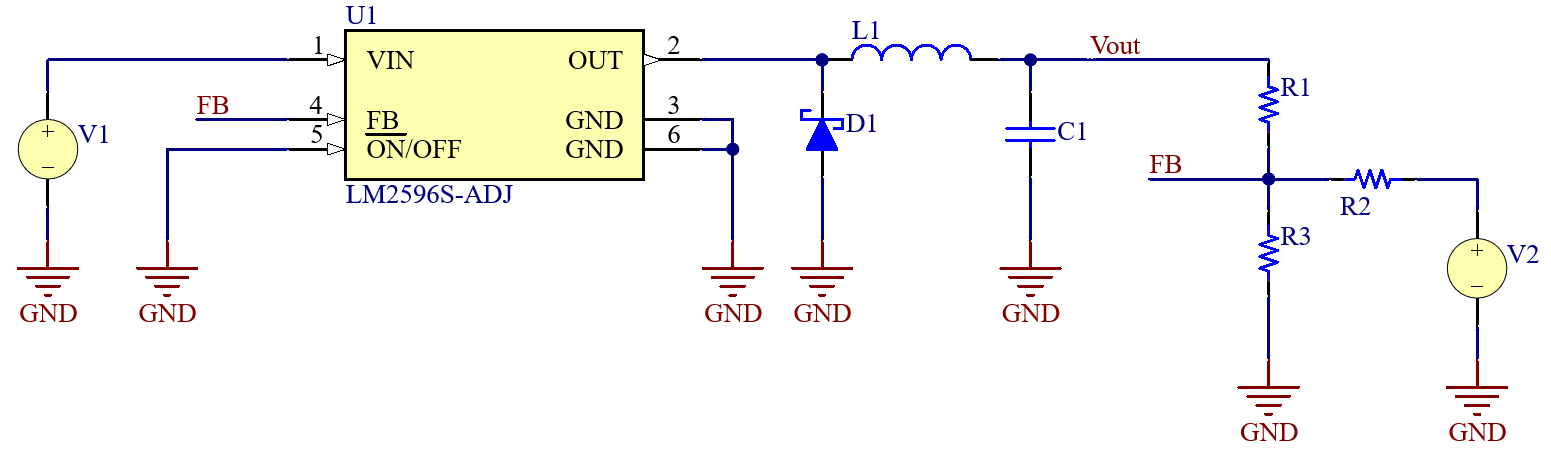
\includegraphics[scale=0.35]{imagenes/buck_control_simplificado.png}
        \caption{Convertidor reductor con realimentación modificación (versión simplificada) }
        \label{fig:buck_modificado}
    \end{figure}

    Para este convertidor se definieron los siguientes parámetros de rendimiento:

    $$ \Delta I = 150 \text{mA} $$
    $$ \Delta V = 1 \text{mV}$$

    Otros parámetros útiles para el diseño de este convertidor serán el voltaje
    de alimentación ($V_g$), así como la frecuencia de conmutación, $f_s$ (dada por la hoja 
    de datos del fabricante), los valores son:

    $$V_g = 12\text{V}$$
    $$ f_s = \frac{1}{T_s} = 150 \text{KHz}$$



    \subsection{Cálculo de resistencias para el circuito de retroalimentación}

    \label{sec:res_ret}

    Para poder determinar en que forma va a variar el voltaje en el nodo $V_{out}$ se realizó un 
    análisis de nodos en el nodo FB correspondiente a la figura \ref*{fig:buck_modificado}, 
    obteniendo la ecuación \ref*{eq:buck_control}.

    \begin{equation}
        V_{FB} = \frac{R_1R_2}{R_1R_2+R_3(R_1+R_2)} V_{out} + \frac{R_1R_3}{R_1R_3+R_2(R_1+R_3)} V_2
        \label{eq:buck_control}
    \end{equation}

    Donde $V_2$ el voltaje aplicado de forma externa para modificar el valor
    de voltaje a la salida. De la ecuación \ref*{eq:buck_control} se puede 
    observar que el valor de $V_{FB}$ es dependiente tanto de $V_2$ como de
    $V_{out}$. 

    Para determinar los valores de las resistencias se armó un sistema de dos ecuaciones,
    fijando los valores de $V_{FB}$,$V_{out}$,$V_2$, y $R_1$. Los dos valores necesarios
    de $V{out}$ se obtuvieron fijando el valor mínimo y máximo que podría tener a la salida
    el convertidor, los cuales fueron de $2.8\text{V}$ y $6.4\text{V}$ de forma que pueda usarse tanto para 
    cargar la celda de batería Li-ion, así como las 4 celdas NiMH. El valor de $V_{FB}$ 
    es el voltaje de referencia del IC LM2596. Los valores del voltaje de control se
    establecieron de forma que, cuando $V_2 = 5\text{V}$ el voltaje a la salida sea de 
    $2.8\text{V}$ mientras que cuando  $V_2 = 0\text{V}$ el voltaje sea de $6.4\text{V}$.
    Por último, se escogió un valor de $750\Omega$ para $R_1$ de forma arbitraria, siguiendo
    la recomendación de la hoja de datos del LM2596.

    Con lo explicado anteriormente, el sistema de ecuaciones a resolver es el siguiente:
    \begin{eqnarray}
        \frac{750R_3}{ 750R_3 + R_2(750 + R_3)} 6.4\text{V} = 1.23\text{V} \\
        \frac{750R_3}{ 750R_3 + R_2(750 + R_3)} 2.8\text{V} + \frac{750R_2}{750R_2+R_3(750+R_2)} 5\text{V} = 1.23\text{V}   
    \end{eqnarray}
    dando como resultado los siguientes valores para $R_2$ y $R_3$:

    $$R_2 = 2596.64\Omega$$ 
    $$R_3 = 3606.44\Omega$$

    Puesto que estos valores no son comerciales, se emplearon valores de resistencias en 
    paralelo, de forma que sea posible aproximar estos valores. Para el valor de $R_2$ 
    se empleó una resistencia de $3\text{K}\Omega$ y $20\text{K}\Omega$ dando como 
    resistencia equivalente $2.608\text{K}\Omega$. De igual forma se utilizó una 
    resistencia de $4.7\text{K}\Omega$ en paralelo con una de $15\text{K}\Omega$ para aproximar
    el valor de $R_3$, dando una resistencia total de $3.578\text{K}\Omega$.

    Al reemplazar en la ecuación \ref{eq:buck_control} los valores para $R_2$ y $R_3$ utilizados, 
    y dando un valor a $V_2$ de $5\text{V}$ se obtiene que el valor de $V_{out}$ es de $2.786\text{V}$
    mientras que si se reemplaza con $V_2 = 0\text{V}$ se obtiene que el valor de $V_{out}$ es de
    $6.431\text{V}$, los cuales son valores aceptables para la carga de ambas baterías,
    de forma que la variación en las resistencias no afecta significativamente
    el rango de operación del convertidor.

    \subsection{Componentes externos del convertidor}

        Los componentes externos necesarios para que el convertidor esté completo, son el 
        diodo $D_1$, el inductor $L_1$, y el capacitor $C_1$ que se muestran en la figura
        \ref{fig:buck_modificado}.

        Para $D_1$ se escogió el diodo 1N5817, el cual es un diodo \textit{
        schotky}, la elección de este componente fue debido a su baja caída de voltaje
        ($0.45\text{V}$ al conducir $1\text{A}$) lo cual minimiza las pérdidas por 
        conducción del mismo, mejorando la eficiencia del convertidor.

        Ya que el valor del inductor es dependiente
        del valor del voltaje a la salida del convertidor es necesario determinar cuál
        sería el valor óptimo. Para ello se definió la función $L(V)$ a partir de las 
        ecuaciones \ref{eq:ripple_L} y \ref{eq:salida_buck}. La función es la siguiente: 

        \begin{equation}
            L(V) = \frac{V_g - V}{2\Delta I}\frac{V}{V_g} T_s
            \label{eq:L_function}
        \end{equation}

        Posteriormente se obtuvo que el valor en
        donde la de derivada de $L(V)$ tiene un valor de cero es en $V = \frac{V_g}{2}$,
        por lo tanto, el valor máximo que tomará $L(V)$ será de 

        $$ L =  \frac{T_sV_g}{8\Delta I}$$
        
        Reemplazando los valores en la ecuación anterior se obtiene que el valor de 
        $L_1$ para el cual se asegura como máximo un rizado de $150 \text{mA}$ en 
        todo el rango de operación, es de $66.6 \mu \text{H}$, por lo que se usó un
        inductor de $68 \mu \text{H}$. Este aumento en el valor del inductor no afecta
        de manera negativa el funcionamiento del convertidor, ya que el valor calculado
        anteriormente unicamente es un límite inferior para el valor del inductor, un 
        valor mas alto reducirá a un mas el rizado en la corriente de salida, lo que 
        mejora el funcionamiento del convertidor.

        Por último, se empleó la ecuación \ref{eq:ripple_C} para obtener el valor 
        de $C_1$, siendo este de $125 \mu\text{F}$, por lo que se utilizó un capacitor
        electrolítico de $220 \mu\text{F}$ debido a que es el siguiente valor comercial 
        más alto disponible. De igual forma que con el inductor, el
        aumento en el valor del capacitor no afecta de manera negativa el funcionamiento
        del convertidor, ya que el valor calculado anteriormente es un límite inferior
        para el valor del capacitor, un valor más alto reducirá a un más el rizado en
        el voltaje de salida.

    \subsection{Componentes adicionales}

        Para asegurar un funcionamiento óptimo en \cite{lm2596}, se aconseja incorporar
        un capacitor en paralelo con la resistencia $R_2$ mostrada en la figura
        \ref{fig:buck_modificado}. La elección del valor de este condensador se basó
        en las pautas proporcionadas en el cuadro \ref{tb:feedforward_cap}. 
        Dado que el voltaje de salida mínimo es de $2.8\text{V}$, se optó por utilizar
        un capacitor de $33\text{nF}$.

        \begin{table}[H]
            \centering
            \begin{tabular}{|c|c|}
                \hline
                Voltaje de salida (V) & Capacitor \\
                \hline
                2 & $33\text{nF}$ \\
                4 & $10\text{nF}$ \\
                6 & $3.3\text{nF}$ \\
                9 & $1.5\text{nF}$ \\
                12 & $1\text{nF}$ \\
                15 & $680\text{pF}$ \\
                24 & $220\text{pF}$ \\
                28 & $220\text{pF}$ \\
                \hline
            \end{tabular}
            \caption{Valores para capacitancia de retroalimentación según \cite{lm2596}
                con respecto al voltaje de salida.}
            \label{tb:feedforward_cap}
        \end{table}



        Otro componente adicional necesario es un capacitor de desacople a la entrada
        del LM2596 para mejorar la estabilidad del voltaje de alimentación. Para su
        selección se empleó como criterio el uso de la figura \ref{fig:rms_cap}. Según
        \cite{lm2596} es necesario asegurar que el capacitor de salida pueda tolerar
        una corriente RMS entre el $50\%$ y $75\%$ de la corriente de salida.
        Para dar un mayor margen, se decidió escoger un capacitor que soporte una corriente
        RMS igual a la corriente máxima esperada, por lo que se escogió un capacitor
        de $470\mu\text{F}$ a $25\text{V}$.

        \begin{figure}[H]
            \centering

            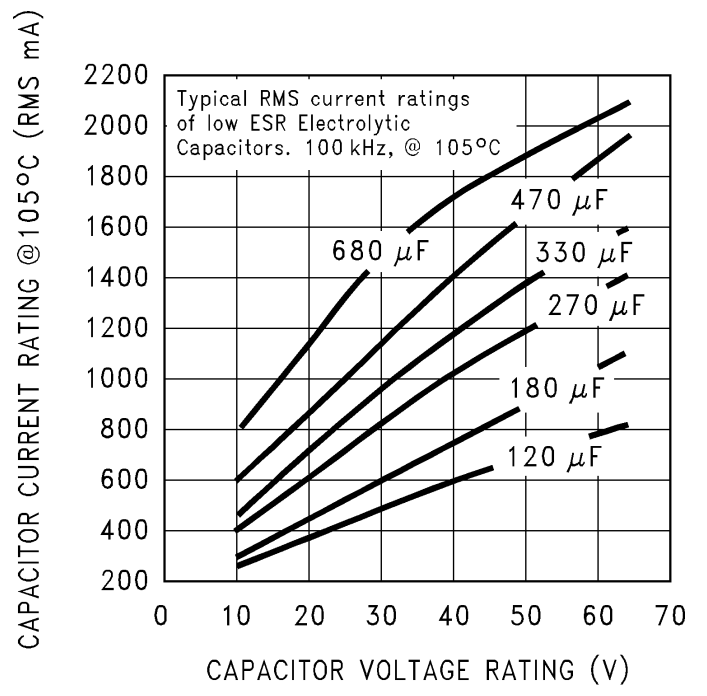
\includegraphics[scale=.4]{imagenes/rms_cap.png}
            \caption{capacidad de corriente RMS}
            \label{fig:rms_cap}

        \end{figure}

        Con todo lo discutido anteriormente, el diseño del convertidor reductor es mostrado
        en la figura \ref{fig:buck_finalizado}.

\begin{figure}[H]
    \centering

    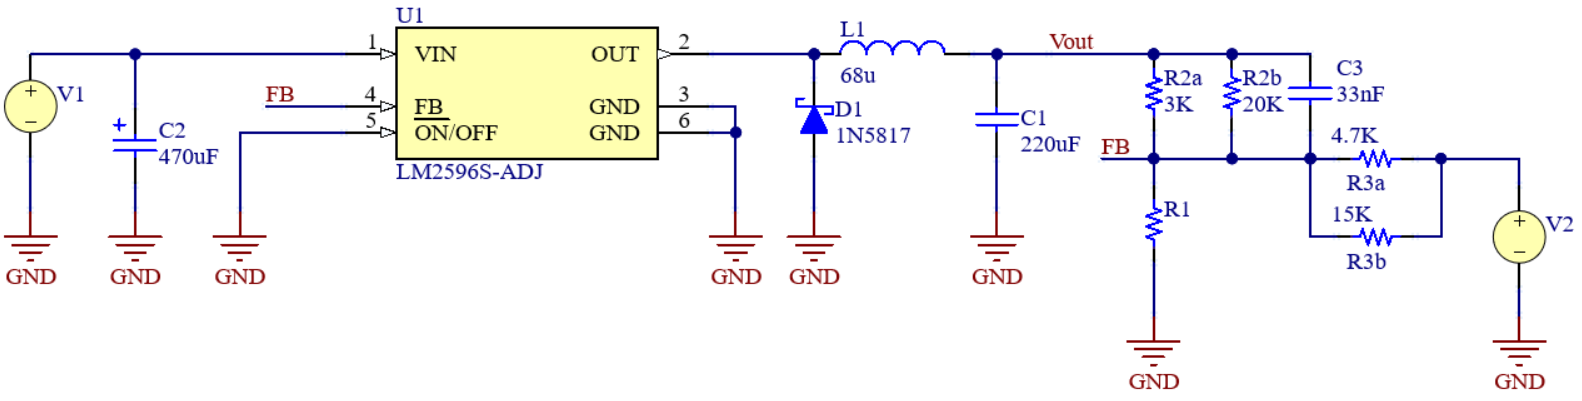
\includegraphics[scale=.45]{imagenes/buck_control_finalizado.png}
    \caption{Diseño del convertidor reductor finalizado}
    \label{fig:buck_finalizado}
\end{figure}

\subsection{Simulación del convertidor diseñado}

Para comprobar el correcto funcionamiento se realizó una simulación del 
convertidor diseñado. Para ello se empleó el simulador LTspice, junto con 
el modelo spice proporcionado por texas instruments para el circuito integrado
LM2596 (descarga disponible en \cite{noauthor_lm2596_nodate}). 

\begin{figure}[H]
    \centering
    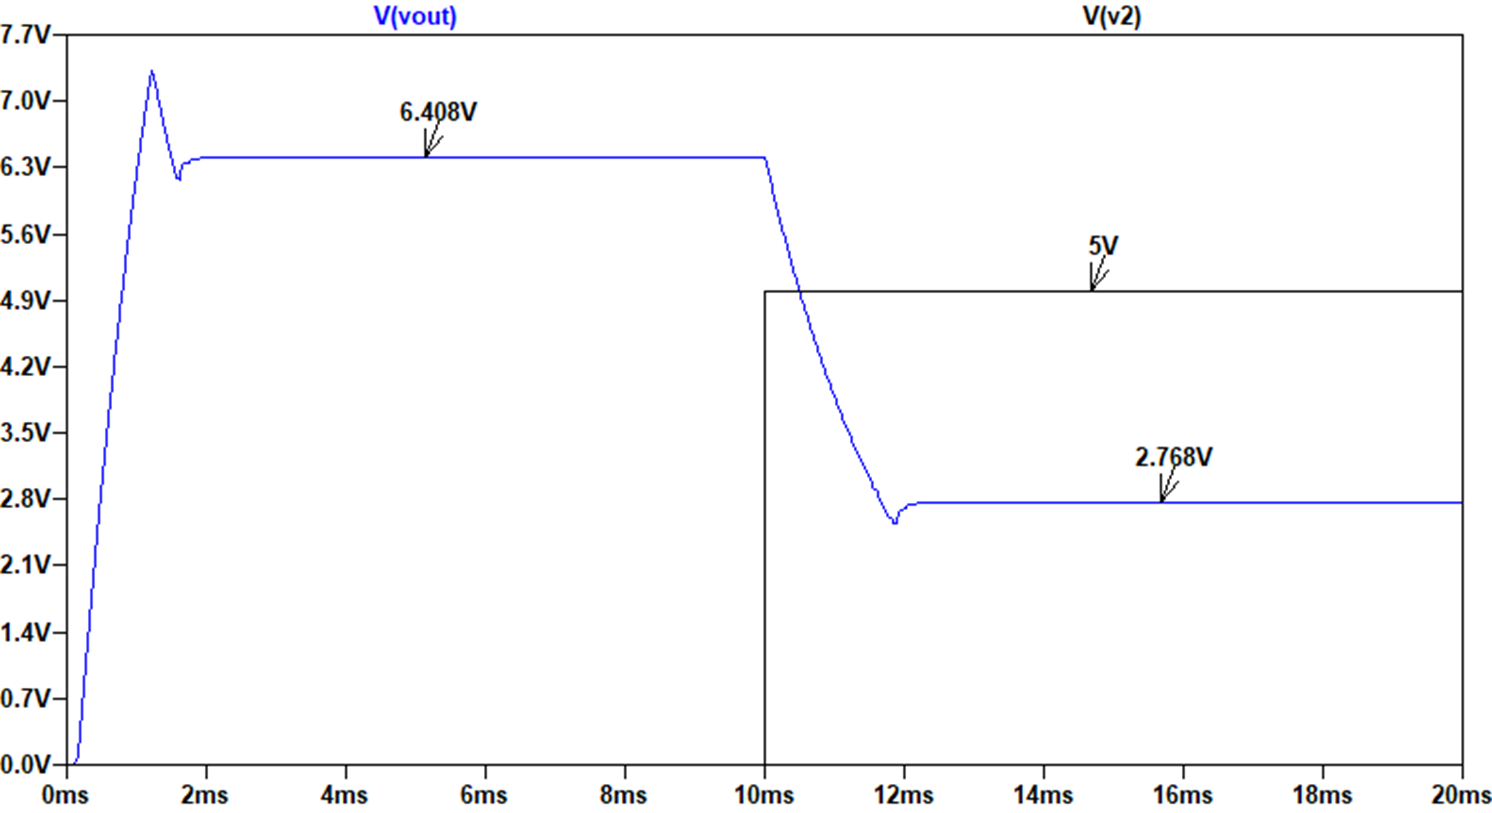
\includegraphics[scale=0.35]{imagenes/resultado_simulacion.png}
    \caption{Respuesta del convertidor (azul) contra el voltaje de control
            (negro).}
    \label{fig:sim_buck}
\end{figure}

En la figura \ref{fig:sim_buck} se muestra la respuesta del convertidor al
aplicar una señal escalón de $5\text{V}$ en la entrada de control. Se puede
observar que cuando el valor en el voltaje de control es de $0\text{V}$
la salida es de $6.408\text{V}$, además
cuando el valor del voltaje de control es de $5\text{V}$ el voltaje a la salida
del convertidor es de $2.768\text{V}$. Los cuales son valores cercanos a los esperados
al momento de realizar el diseño. 

Adicionalmente se puede observar que el rizado en el voltaje de salida del 
convertidor no es observable a la escala de voltaje en el que se está, esto debido
al uso de un valor más alto al calculado tanto para el inductor como para el 
capacitor del convertidor.

                                                                
\subsection{Prueba física del circuito}

Como último paso se realizó el diseño de un circuito impreso para probar el 
funcionamiento del circuito, en la figura \ref{fig:buck_pcb} se muestra la capa
superior e inferior del PCB.

\begin{figure}[H]
    \centering
    \begin{subfigure}{0.45\linewidth}
        \centering
        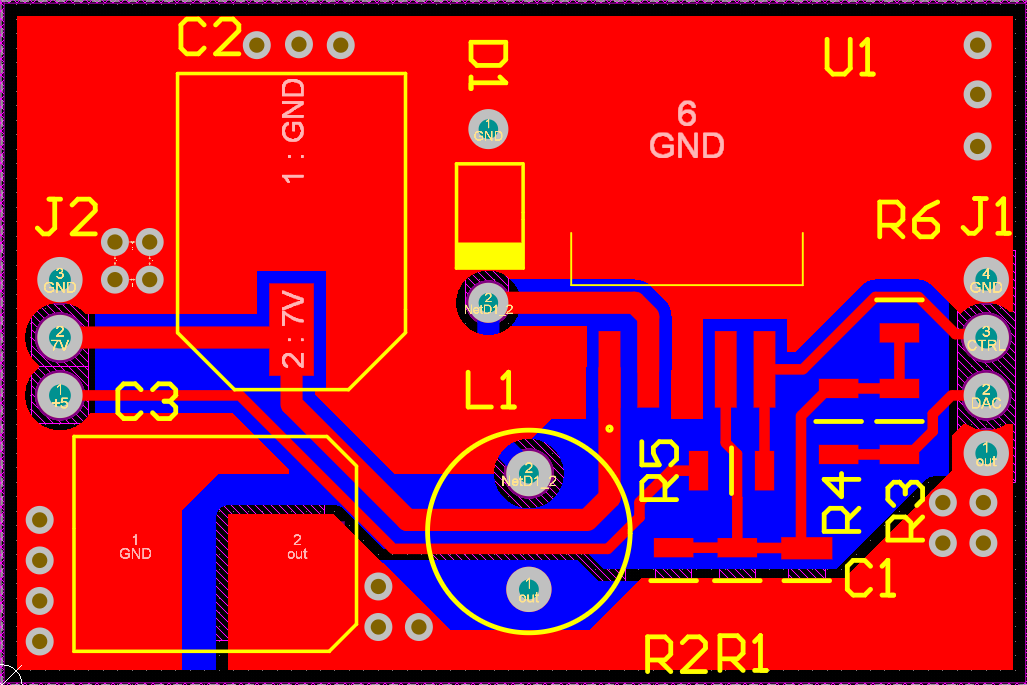
\includegraphics[scale=0.3]{imagenes/top_buck.png}
        \caption{Capa superior}
    \end{subfigure}
    \begin{subfigure}{0.45\linewidth}
        \centering
        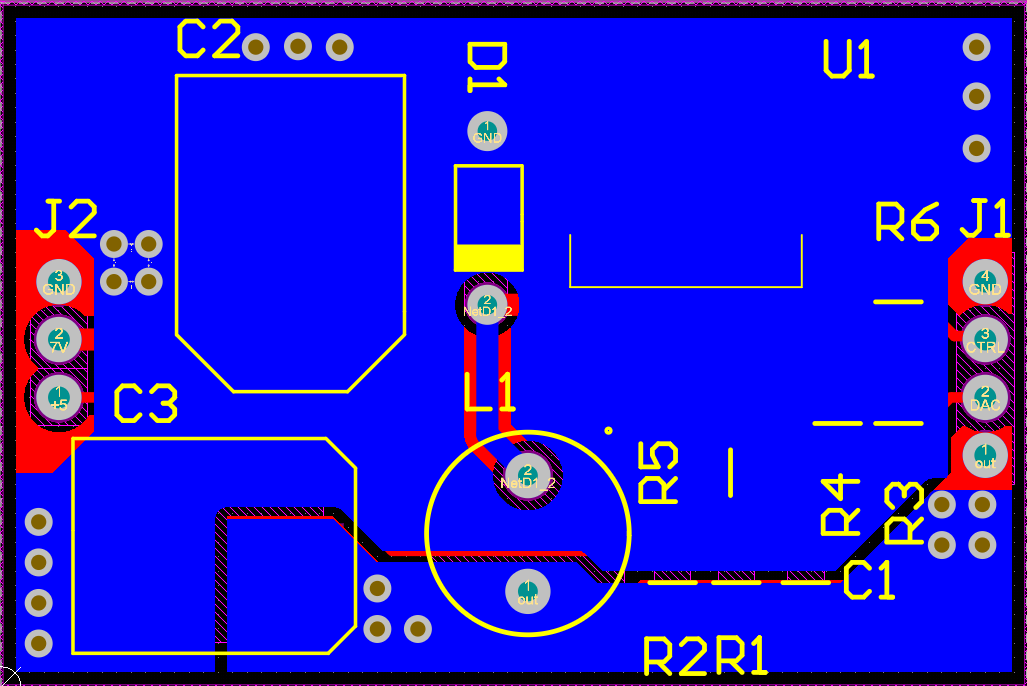
\includegraphics[scale=0.3]{imagenes/bottom_buck.png}
        \caption{Capa inferior}
    \end{subfigure}
    \vfill
    \begin{subfigure}{0.45\linewidth}
        \centering
        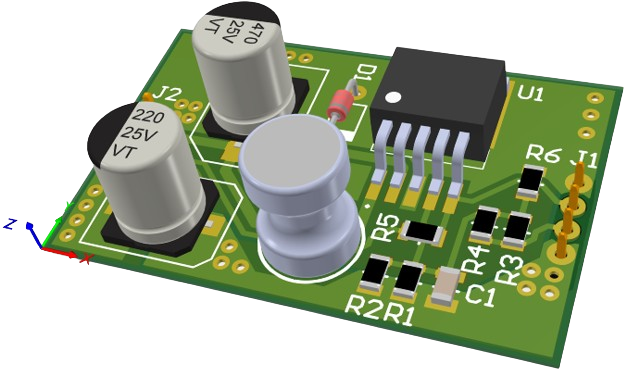
\includegraphics[scale=0.3]{imagenes/3d_buck.png}
        \caption{Vista 3D}
    \end{subfigure}
    \begin{subfigure}{0.45\linewidth}
        \centering
        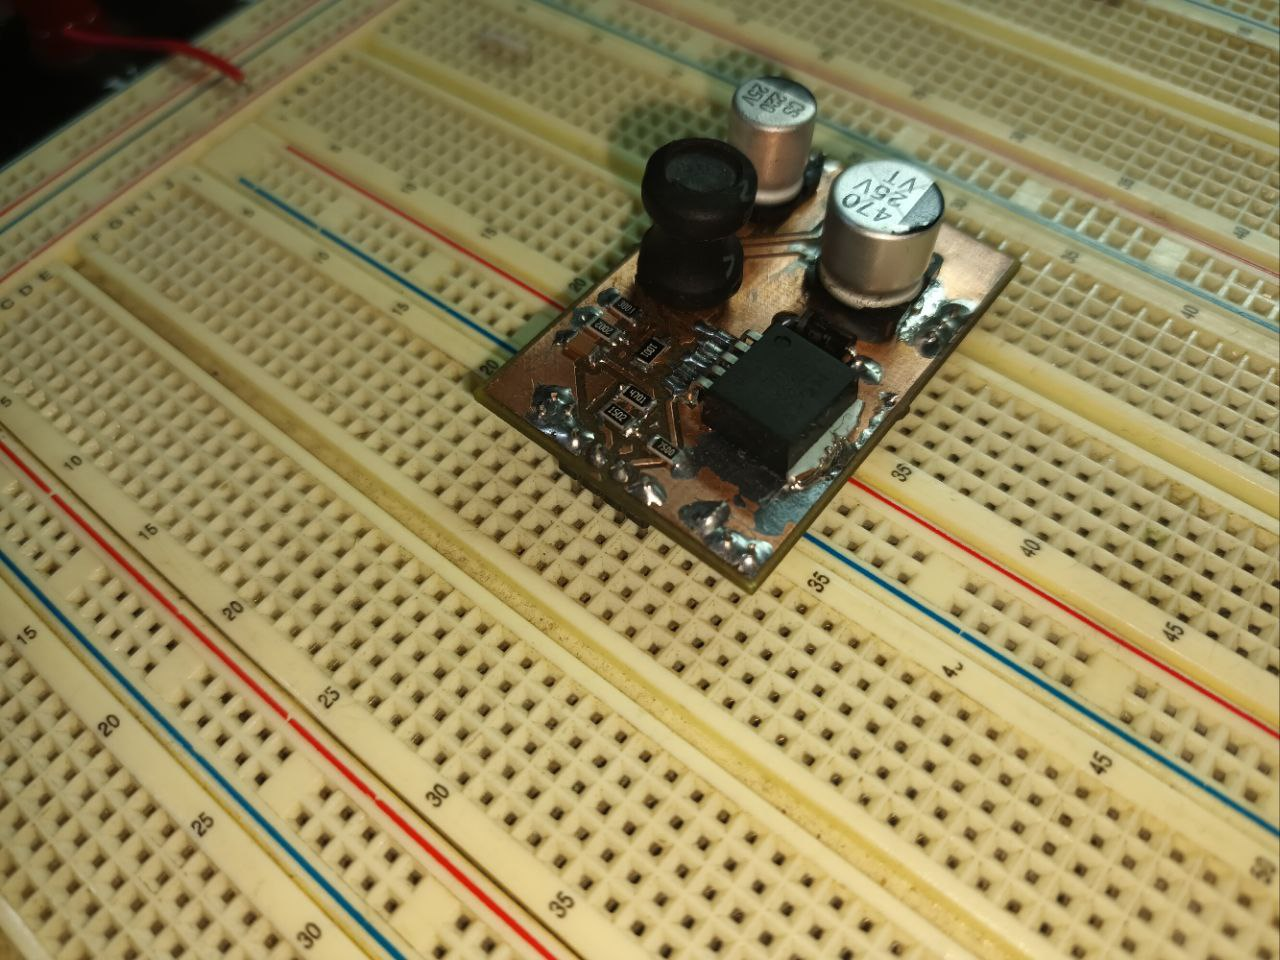
\includegraphics[scale=0.12]{imagenes/circuit_phis1.jpg}
        \caption{PCB ensamblada}
    \end{subfigure}
    \caption{Diseño del PCB para el convertidor reductor}
    \label{fig:buck_pcb}
\end{figure}

Debido a que se manejan corrientes de hasta $1.5\text{A}$ es necesario que el
diseño del PCB sea capaz de manejar dicha corriente, para ello se empleó una 
calculadora de ancho de pistas \cite{noauthor_pcb_nodate}, con el cual se 
determinó que el ancho de las pistas debe ser de $0.53\text{mm}$ como mínimo,
esto tomando en cuenta que se estará usando un cobre con espesor de 1oz, y que
el maximo aumento de temperatura permitido es de 10\textordmasculine C. 

Se programó el microcontrolador ATmega328p para que genere una señal 
cuadrada de $5\text{V}$ con un periodo de 10 segundos en el pin PB1,
la cual se conectó a la entrada de control del convertidor. Al medir el voltaje
en la salida se obtuvo que el voltaje cuando se tienen $5\text{V}$ en la entrada
de control es de $2.76\text{V}$, mientras que cuando se tiene $0\text{V}$
en la entrada de control el voltaje a la salida es de $6.40\text{V}$, estos 
valores son cercanos a los esperados, por lo que el convertidor diseñado
funciona de forma correcta.

El circuito construido en protoboard para la prueba del convertidor se muestra
en la figura \ref{fig:prueba_buck}.

\begin{figure}[H]	
    \centering
    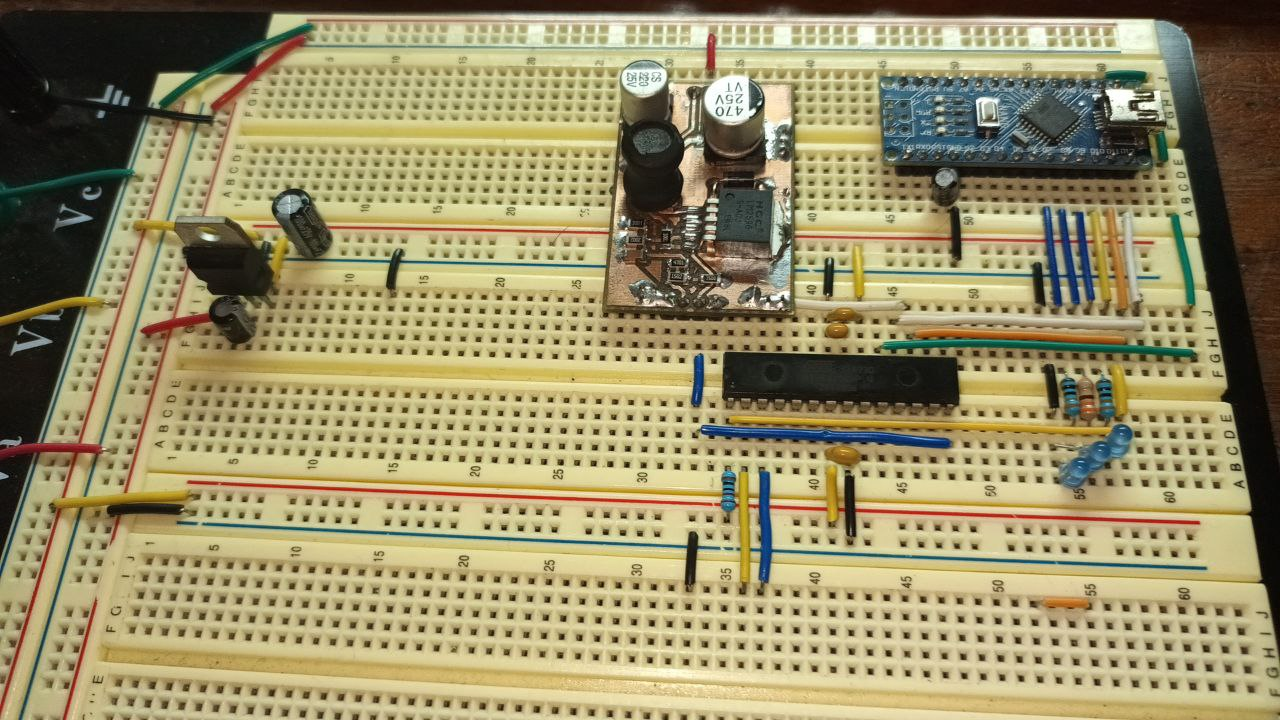
\includegraphics[scale=0.2]{imagenes/prueba_buck.jpg}
    \caption{Circuito para prueba del convertidor reductor (Arduino Nano únicamente
    para programar el ATmega328p)} 
    \label{fig:prueba_buck}
\end{figure}

El código empleado en la prueba se muestra a continuación.

\begin{table}[H]
    \begin{lstlisting}
        #define F_CPU 8000000UL
        #include <avr/io.h>
        #include <util/delay.h>


        int main(void) {
                // ----     IO CONFIG  ---------
            DDRB = 0b00000011; // PB[7:2] input, PB1 out, PB0 out
            
            PORTB = 0b0000000; //activar PB0
            while (1) {
                PORTB |= 1<<1; //PB1 en 1
                _delay_ms(10000);
                PORTB &= ~(1<<1); //PB1 en 0
                _delay_ms(10000);
            }
        }

    \end{lstlisting}
    \caption{Código para prueba del convertidor reductor}
\end{table}

    
    \section{Sensor de corriente}

    Para poder usar el convertidor reductor explicado en la sección
    \ref{sec:buck_design} es necesario medir la corriente que se
    está entregando a la batería. Para ello se diseñó un sensor de corriente
    basado en el amplificador operacional TL082.

    El sensor tiene 2 componentes principales, el amplificador diferencial y 
    la resistencia de sensado. El amplificador diferencial se encarga de 
    amplificar la diferencia de potencial entre los terminales de la resistencia
    de sensado, la cual es proporcional a la corriente que circula por la misma.
    La resistencia de sensado tiene un valor de $15 \text{m}\Omega$, con una
     tolerancia de $\pm 5\%$.

    Para poder medir una corriente máxima de $1.5\text{A}$ se escogió que 
    la ganancia para el amplificador diferencial (ver figura \ref{fig:ampDif})
    sea de $200\text{V/V}$, por lo que la salida del sensor será de
    $4.5\text{V}$ cuando la corriente sea de $1.5\text{A}$. Para obtener
    la ganancia deseada, se calcularon los valores de resistencia 
    necesarios utilizando la Ecuación \ref{eq:ampDifSimp}, fijando 
    el valor de $R_2$ en
    $1.5\text{K}\Omega$, obteniendo que el valor de $R_4$ debe ser de 
    $300\text{K}\Omega$. Debido a la  simplificación del circuito hecha en la 
    sección \ref{sec:ampDif} el valor de $R_1$ debe ser de $1.5\text{K}\Omega$
    y el valor de $R_3$ debe ser de $300\text{K}\Omega$. El sensor de corriente 
    diseñado se muestra en la figura \ref{fig:sensor_corriente}.

    \begin{figure}[H]
        \centering
        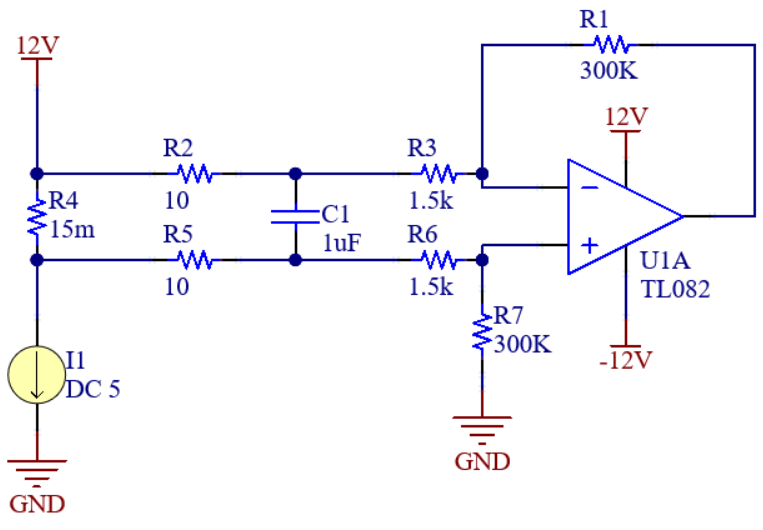
\includegraphics[scale=0.5]{imagenes/current_sensor.png}
        \caption{Sensor de corriente diseñado}
        \label{fig:sensor_corriente}
    \end{figure}

    con lo explicado anteriormente, el sensor tiene una ganancia final de 
    $3\text{V/A}$, la ecuación \ref{eq:sensor} describe la relación entre
    la corriente que circula por la resistencia de sensado y el voltaje de salida
    del amplificador diferencial.

    \begin{equation}
        V_{out} = 3I_1
        \label{eq:sensor}
    \end{equation}
    
    Para la alimentación del sensor es necesario un mínimo de $\pm7\text{V}$ en
    los pines de alimentación del amplificador operacional TL082, esto por dos 
    motivos, el primero es que el voltaje de salida del sensor es de $4.5\text{V}$
    cuando la corriente es de $1.5\text{A}$ tomando en cuenta que este opamp 
    no es del tipo \textit{rail to rail}, por lo que el voltaje de salida no
    puede ser igual al voltaje de alimentación, y el segundo motivo es que el
    voltaje en modo común de este amplificador tiene como limite superior el
    voltaje de alimentación positivo, por lo que es necesario que el voltaje 
    de alimentación sea mayor que el voltaje máximo de que recibirá en sus entradas,
    que para este caso es de $6.4\text{V}$. Para alimentar el sensor se empleó
    una alimentación simétrica de $\pm 12\text{V}$.
    
    \subsection{Mediciones del Sensor de corriente}

    Para comprobar el correcto funcionamiento del sensor de corriente diseñado
    se realizaron mediciones para varios niveles de corriente. Para ello se
    empleó una fuente de voltaje simétrica a $\pm7\text{V}$, y se utilizaron resistencias de entre 
    $4\Omega$ y $30\Omega$ para simular la carga de la batería. Los resultados 
    obtenidos son mostrados en el cuadro \ref{tb:mediciones_sensor}. 

\begin{table}[H]
    \centering
    \begin{tabular}{|c|c|c|c|}
        \hline
    Corriente medida & Salida del sensor (V) & Valor Ideal (V) & Error (\%) \\
    \hline
    0.241            & 0.815                 & 0.795           & 2.48       \\
    0.480            & 1.546                 & 1584            & 2.40       \\
    0.713            & 2.270                 & 2.353           & 3.52       \\
    0.933            & 2.945                 & 3.079           & 4.35       \\
    1.143            & 3.592                 & 3.772           & 4.77       \\
    1.354            & 4.24                  & 4.47            & 5.11       \\
    1.564            & 4.88                  & 5.16            & 5.43 \\
     \hline     
    \end{tabular}

    \caption{Valores de salida del sensor de corriente diseñado}
    \label{tb:mediciones_sensor}
    \end{table}


    En la figura \ref{fig:mediciones_sensor} se muestra el circuito construido
    en protoboard para la medición de los valores presentados anteriormente.

    \begin{figure}[H]
        \centering
        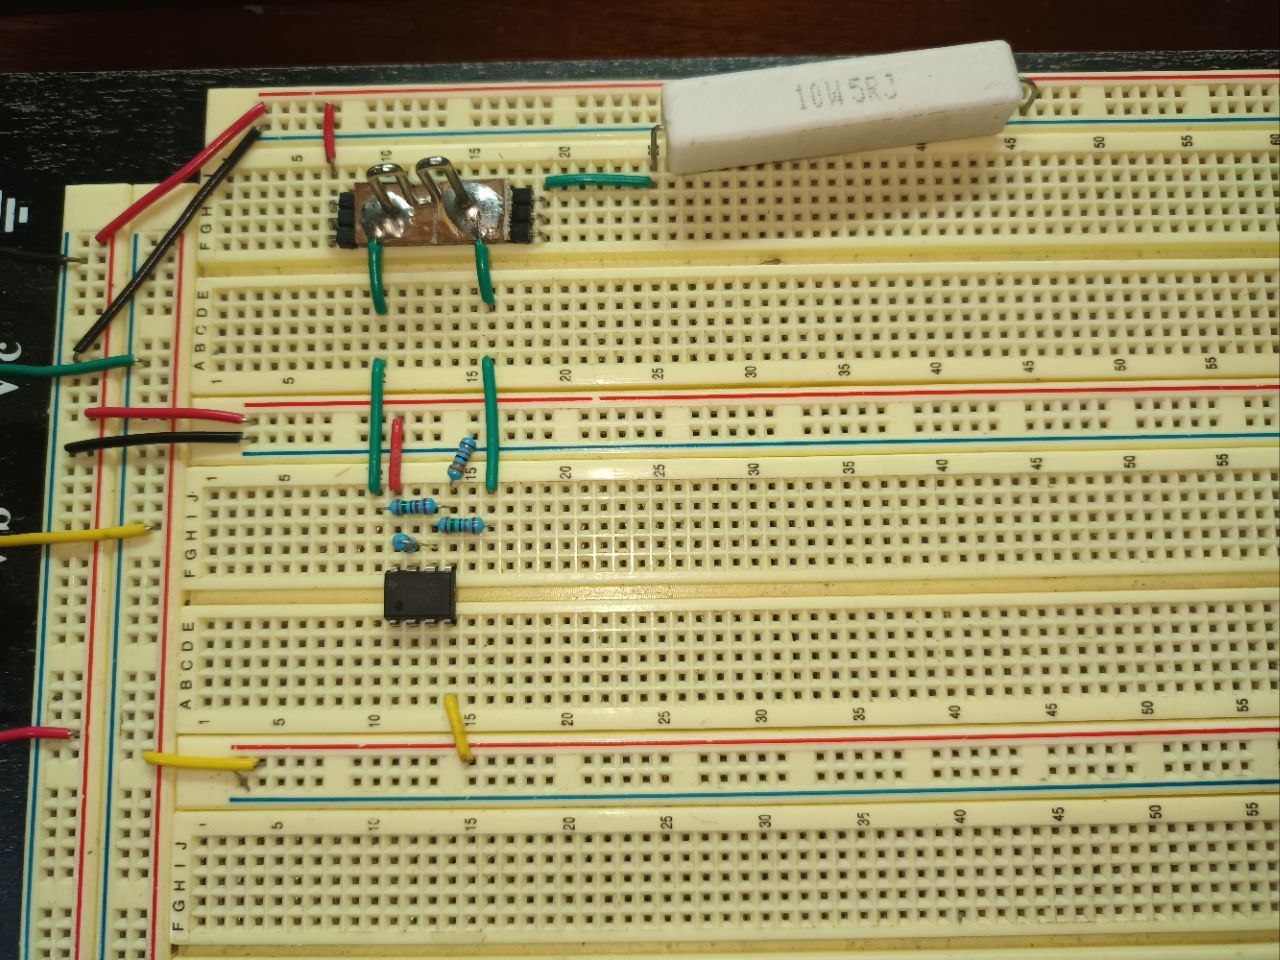
\includegraphics[scale=0.2]{imagenes/prueba_sensor.jpg}
        \caption{Circuito para medición del sensor de corriente}
        \label{fig:mediciones_sensor}
    \end{figure}


    \section{Conversor digital a analógico (DAC)}

    Para controlar el voltaje de salida del convertidor reductor es necesario
    poder generar un voltaje de control de forma digital. Para ello se diseñó
    un conversor digital a analógico (DAC) utilizando un filtro RC de primer
    orden y un amplificador operacional en modo seguidor de voltaje. El DAC
    propuesto se muestra en la figura \ref{fig:dac}.

    \begin{figure}[H]
        \centering
        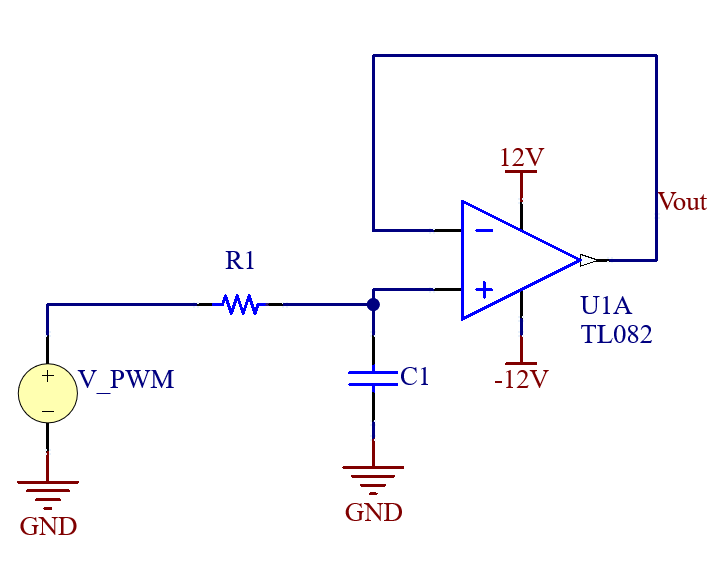
\includegraphics[scale=0.5]{imagenes/dac_disenio.png}
        \caption{DAC propuesto}
        \label{fig:dac}
    \end{figure}

    Ya que para la generación de la de PWM se utilizó el módulo PWM1 (debido
    a que este es el que presenta una mayor resolución) del ATmega328p, con el 
    cual se puede generar una señal PWM con una resolución de 10 bits, que en
    conjunto con una frecuencia de operación para el microcontrolador de $8\text{MHz}$
    se obtiene una frecuencia de PWM de $7.81\text{KHz}$, se determinó que la 
    frecuencia de corte del filtro RC sea de $70\text{Hz}$, de forma el armónico
    de mayor magnitud (el cual es el de frecuencia $7.81\text{KHz}$) sea atenuado
    en $-40\text{dB}$. 

    La frecuencia de corte para el filtro RC está dada por la ecuación \ref{eq:fc_dac},
    donde $R$ es el valor de la resistencia y $C$ es el valor del capacitor, mostrados
    en la figura \ref{fig:dac}.

    \begin{equation}
        f_c = \frac{1}{2\pi RC}
        \label{eq:fc_dac}
    \end{equation}

    Se fijó el valor del capacitor en $0.1\mu\text{F}$, por lo que el valor de la
    resistencia es de $22.7\text{K}\Omega$, por lo que se utilizará el valor 
    de resistencia comercial más cercano, el cual es de $22\text{K}\Omega$.
    Este cambio realizado en valor de la resistencia no afecta
    significativamente el comportamiento del filtro, ya que el objetivo 
    principal del mismo es atenuar los armónicos de la señal PWM, que es 
    dos órdenes de magnitud mayor a la frecuencia de corte del filtro.

    \subsection{Simulación del DAC}

    Para comprobar el correcto funcionamiento del DAC diseñado se realizó una
    simulación del mismo. Para ello se empleó el simulador LTspice, junto con
    el modelo spice proporcionado por texas instruments para el circuito integrado
    TL082 (descarga disponible en \cite{noauthor_tl082_nodate}). Para ello se 
    generó una señal pwm de $15.625KHz$ la cual varía su ciclo de trabajo 
    de forma que en la salida se obtenga una señal senoidal de $10\text{Hz}$. 
    En la figura
    \ref{fig:sim_dac} se muestra la respuesta del DAC ante la señal PWM de entrada.

    \begin{figure}[H]
        \centering
        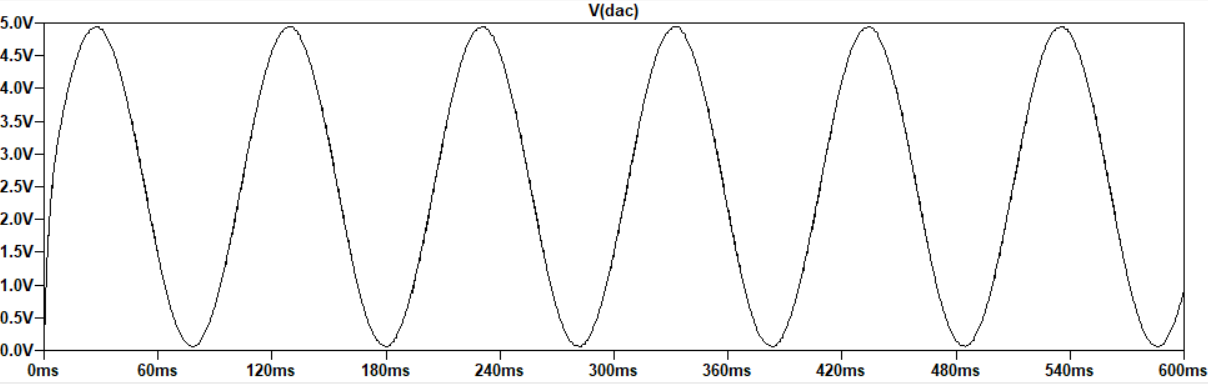
\includegraphics[scale=0.45]{imagenes/dac_out.png}
        \caption{Respuesta del DAC ante una señal PWM}
        \label{fig:sim_dac}
    \end{figure}

    En la figura \ref{fig:sim_dac} se puede observar que la señal de salida
    del DAC es una señal senoidal de $10\text{Hz}$, que es lo esperado ya 
    que la señal PWM varía su ciclo de trabajo también de forma senoidal.
    Además, se puede observar que el valor máximo de la señal de salida es
    de $5\text{V}$, mientras que el valor mínimo es cercano $0\text{V}$
    comprobando que el DAC funciona de forma correcta, ya que la señal PWM
    varía su ciclo de trabajo entre $0\%$ y $100\%$, haciendo que el valor 
    DC de la señal PWM varíe también entre $0\text{V}$ y $5\text{V}$.

    Adicionalmente en las figuras \ref{fig:sim_dac_fft} y \ref{fig:sim_dac_fft_in}
    se muestra la transformada de Fourier discreta (DFT) de la señal de salida
    del DAC, y de la señal PWM de entrada respectivamente. Se puede ver 
    que los armónicos correspondientes a la señal PWM de entrada son atenuados
    hasta el punto de que no son visibles en la DFT de la señal de salida del
    DAC, lo cual es lo esperado, ya que el filtro RC tiene una frecuencia de corte
    de $72\text{Hz}$, mientras que la frecuencia de la señal PWM es de 
    $15.625\text{KHz}$.

    \begin{figure}[H]
        \centering
        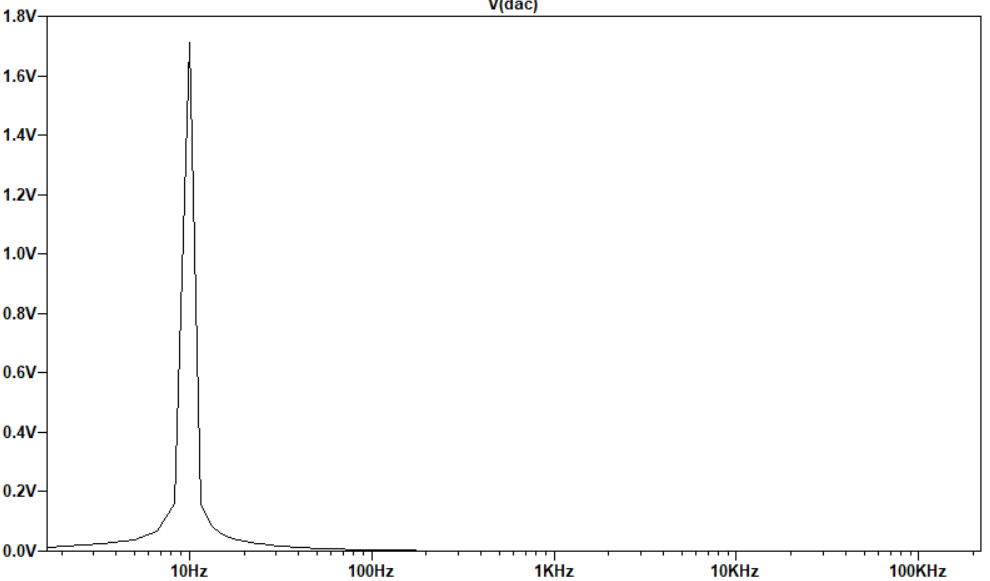
\includegraphics[scale=0.45]{imagenes/fft_dac_salida.png}
        \caption{DFT de la señal de salida del DAC}
        \label{fig:sim_dac_fft}
    \end{figure}

    \begin{figure}[H]
        \centering
        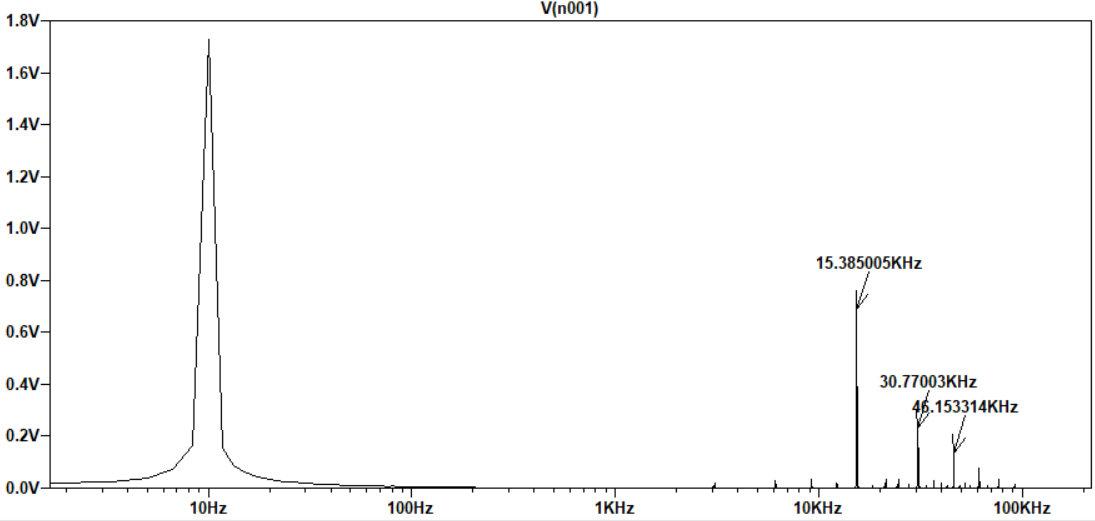
\includegraphics[scale=0.45]{imagenes/fft_dac_pwm.png}
        \caption{DFT de la señal PWM de entrada}
        \label{fig:sim_dac_fft_in}
    \end{figure}

    \subsection{Pruebas con DAC}

    Para comprobar el correcto funcionamiento del DAC diseñado se realizó una
    prueba del DAC, en la cual se generaró 2 señales, una senoidal y una triangular,
    empleando el DAC y el codigo mostrado en el apéndice \ref{sec:codigo_dac} (el cual 
    se puede ubicar dentro de los archivos del proyecto de MPLAB nombrado como
    DAC\_test.X, dentro de la carpeta nombrada Charge\_system\_firmware).
     En la figura \ref{fig:dac_test_sine}
    se muestra el resultado de la prueba.
    
     \begin{figure}[H]
        \centering

        \begin{subfigure}{0.45\textwidth}
            \centering
            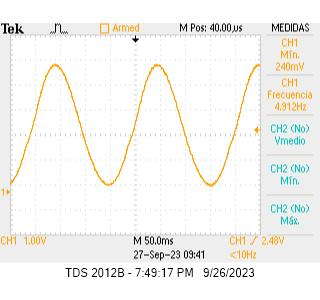
\includegraphics[scale=0.8]{imagenes/Sine.jpg}
            \caption{Señal senoidal}
        \end{subfigure}
        \begin{subfigure}{0.45\textwidth}
            \centering
            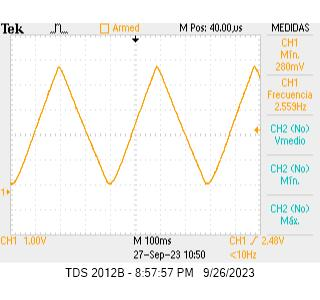
\includegraphics[scale=0.8]{imagenes/Triangular.jpg}
            \caption{Señal triangular}
        \end{subfigure}

        \caption{Señal seno y triangular generadas con el DAC}
        \label{fig:dac_test_sine}
     \end{figure}

     Se puede observar que ambas señales
     tienen una amplitud de $5\text{V}$, y que la señal senoidal tiene una frecuencia
     de $4.91\text{Hz}$, mientras que la señal triangular tiene una frecuencia de
     $2.56\text{Hz}$. La razon por la cual las frecuencias de las señales generadas
     son bajas es debido a la frecuencia de corte del filtro RC, que es de $72\text{Hz}$,
     por lo que señales de mayor frecuencia son atenuadas, hecho que no afecta 
     al sistema de carga multiquímica, ya que la el cambio de voltaje de voltaje 
     en ambas baterias se realiza de forma lenta, por lo que no es necesario
     generar señales de alta frecuencia.
 

    \section{Multiplicador de Voltaje}

    Debido a que el sensor de corriente y el DAC diseñados necesitan una
    alimentación simétrica de $\pm 7\text{V}$ (como mínimo), se diseñó 
    un multiplicador de voltaje basado en el circuito \textit{negative 
    Dickson charge pump} presentado en la sección \ref{sec:charge_pump}.


    Puesto que este necesita de una señal cuadrada, se utilizó un inversor
    elaborado con un transistor BJT , en cascada con una etapa de salida 
    \textit{push-pull}. El inversor es empleado para generar una señal
    cuadrada de amplitud $12\text{V}$ a partir de una señal cuadrada 
    de $5\text{V}$, mientras que la etapa \textit{push-pull}
    es utilizada para aumentar la corriente de salida del inversor, de forma
    que sea capaz de alimentar el multiplicador de voltaje. El circuito
    se muestra en la figura \ref{fig:inversor}.
    
    \begin{figure}[H]
        \centering
        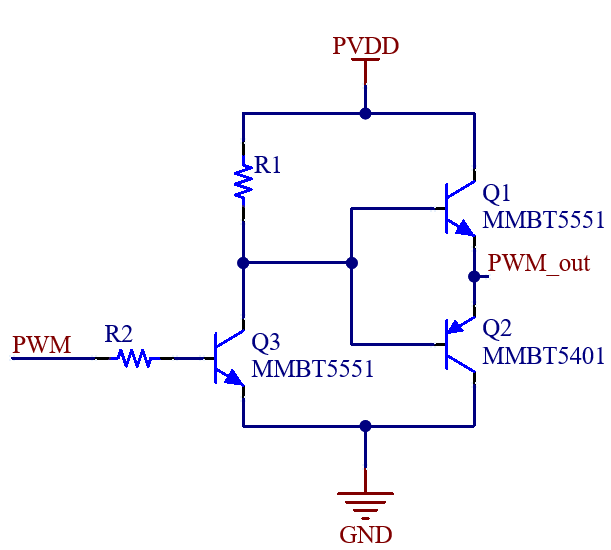
\includegraphics[scale=0.5]{imagenes/clk_gen.png}
        \caption{Inversor utilizado para generar la señal cuadrada}
        \label{fig:inversor}
    \end{figure}

    Para determinar los valores de $R_1$ y $R_2$
    se asumió que el voltaje entre base y emisor ($v_{be}$) del transistor $Q_3$
    es de $1\text{V}$  y que la ganancia en corriente del 
    transistor $Q_3$ es de $10$ \cite{mmtb5551}. Con lo anterior, se fijó el 
    valor de $R_2$ en $1\text{K}\Omega$, por 
    lo que la corriente en la base de $Q_3$ es de $I_b = 4\text{mA}$, y el valor
     esperado para la corriente de colector es de $I_c = 40\text{mA}$.

    Para que este transistor actúe como un inversor es necesario que 
    el transistor $Q_3$ se encuentre alternando entre
    las regiones de corte y saturación. Para ello es necesario
    que el producto $I_cR_1$ sea mayor al voltaje en el nodo PVDD, el cual
    es de $12\text{V}$:
    
    $$
        I_cR_1 > 12\text{V}
    $$
    
   
    $$
        R_1 > \frac{12\text{V}}{40\text{mA}} = 300 \Omega
    $$

    
    Por lo que se utilizó un valor de $R_1 = 1\text{K}\Omega$. Esta señal es 
    pasada en la etapa \textit{push-pull} para aumentar la corriente de salida
    del inversor,asi como disminuir la impedancia, de forma que sea 
    capaz de alimentar el multiplicador de voltaje.

    Para el diseño del multiplicador de voltaje se estableció que la 
    el valor de $C_1$ y $C_2$ sea de
    $1\mu\text{F}$, que el valor de salida requerido debe ser menor o igual
    a $-7\text{V}$ y el número de etapas($N$) es igual a 1. En la 
    ecuación \ref{eq:dickson_charge_neg}  se toma en cuenta la
    capacitancia parásita de los diodos ($C_s$), para el diseño se asumió
    que estas capacitancias no son significativas en comparación con 
    $C_1$ y $C_2$,por lo que se asume $C_s = 0$.
    Con lo anterior, la ecuación \ref{eq:charge_pump} se simplifica a la
    ecuación \ref{eq:charge_pump_simp}. En la figura \ref{fig:charge_pump_dis}
    se muestra el circuito diseñado.

    \begin{figure}[H]
        \centering
        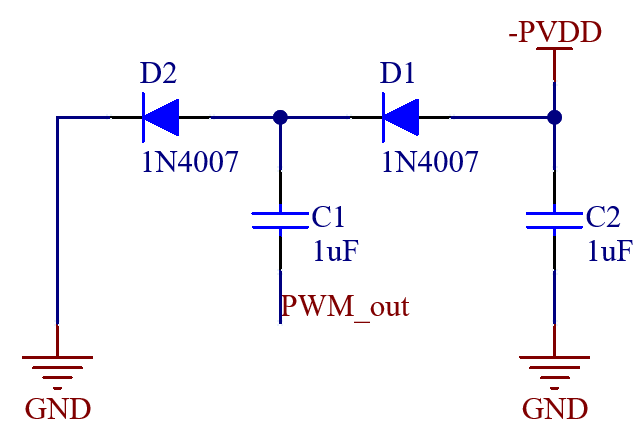
\includegraphics[scale=0.5]{imagenes/dickson_charge.png}
        \caption{Circuito diseñado para el multiplicador de voltaje}
        \label{fig:charge_pump_dis}
    \end{figure}

    \begin{equation}
        V_{out} = -\left(V_\Phi - V_D - \frac{I_{out}}{Cf}  \right)
        \label{eq:charge_pump_simp}
    \end{equation}

    Para determinar la frecuencia de operación, se utilizó la ecuación 
    \ref{eq:charge_pump_simp}, junto con la desigualdad 
    $V_{out} \leq -7\text{V}$, obteniendo la ecuación 
    \ref{eq:charge_pump_simp2}.

    \begin{equation}
        -\left(V_\Phi - V_D - \frac{I_{out}}{Cf}\right) \leq -7\text{V}
        \label{eq:charge_pump_simp2}    
    \end{equation}

    Para la amplitud de la señal cuadrada se utilizó el valor de 
    $V_\Phi = 12 \text{V}$, mientras que para 
    el valor de $V_D$ se utilizó el valor de $0.7\text{V}$, y se estimó que
    la corriente de salida del multiplicador de voltaje es de $10\text{mA}$.
    Despejando para la frecuencia se obtiene la ecuación \ref{eq:charge_pump_simp3}.

    \begin{equation}
        f \geq \frac{I_{out}}{C(V_\Phi - V_D - V_{out})}
        \label{eq:charge_pump_simp3}
    \end{equation}

    Reemplazando los valores en la ecuación \ref{eq:charge_pump_simp3} se obtiene
    la frecuencia de operación del multiplicador de voltaje debe de ser 

        $$
            f \geq \frac{10\text{mA}}{1\mu\text{F}(12\text{V} - 0.7\text{V}
             - 7\text{V})} \approx 2.325\text{KHz}
        $$

    Ya que este es un valor mínimo para la frecuencia de operación, al utilizar
    una frecuencia mayor se obtendrá un voltaje de salida mayor, por lo que se
    utilizó una frecuencia de operación de $7.81\text{KHz}$, la cual es la
    frecuencia de la señal PWM generada por el microcontrolador. 


    \section{multiplexor de potencia}

    Para la selección de la batería que proporcionará la alimentación al agente
    robótico, asi como para la selección de la batería que se cargará se diseñó
    un multiplexor de potencia empleando transistores MOSFET canal P, en 
    configuración \textit{back to back} como se muestra en la figura \ref{fig:power_switch}.

    \begin{figure}[H]
        \centering
        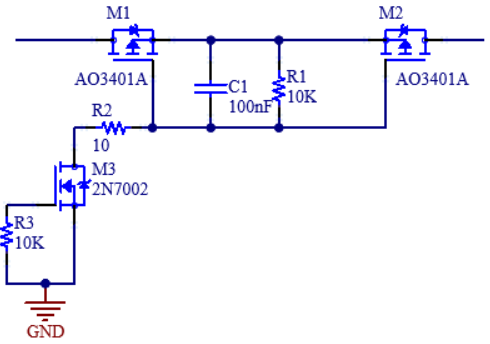
\includegraphics[scale=0.5]{imagenes/power_switch.png}
        \caption{Multiplexor de potencia}
        \label{fig:power_switch}
    \end{figure}

    En el conmutador de la figura \ref{fig:power_switch} se puede observar que se
    emplearon 2 transistores MOSFET caddnal P, de modelo AO3401, estos fueron
    seleccionados debido a que tienen una corriente de \textit{drain} máxima de
    $4\text{A}$, y una resistencia de \textit{drain} a \textit{source} de 
    $0.06\Omega$, lo cual permite que el multiplexor tenga una caída de tensión
    mínima cuando se encuentre en conducción, y un aumento de temperatura mínimo
    debido a la disipación de potencia \cite{a_AO3401}.

    La resistencia $R_1$ tiene como función asegurar que el voltaje 
    entre \textit{gate} y \textit{source} del transistor MOSFET sea de $0\text{V}$,
    cuando el transistor M3 no se encuentre en conducción, asegurando que 
    el conmutador no se encuentre en conducción cuando no se requiera. Los componentes 
    $R_2$ y $C_1$ tienen como función limitar la corriente drenada \textit{gate} de
    los transistores MOSFETs M1 y M2 de forma que se evite dañar los transistores
    cuando se realice el cambio de estado del conmutador, mientras que el propósito
    de la resistencia $R_3$ evitar que la terminal \textit{gate} del transistor
    M3 se encuentre en un estado flotante.

    Para el multiplexor encargado de seleccionar la batería que alimentará al
    agente robótico se utilizó un conmutador como el mostrado en la figura
    \ref{fig:power_switch}, en conjunto con el circuito interno posee el 
    Pololu 3pi+, que permite conectar y desconectar la batería NiMH integrada.

    Para el multiplexor encargado de seleccionar la batería que se cargará se
    emplearon 2 conmutadores como el mostrado en la figura \ref{fig:power_switch},
    el controlador que se describe en la sección \ref{sec:controlador} se encarga
    de seleccionar la batería que se cargará, y de seleccionar la batería que
    alimentará al agente robótico.

    Ambos multiplexores fueron diseñados para tener un funcionamiento manual, 
    es decir, que el microcontrolador será el encargado de seleccionar la batería
    que se cargará, y la batería que alimentará al agente robótico, no existiendo
    un comportamiento automático para la selección de las baterías.

    \subsection{Pruebas del conmutador de potencia}

    Para comprobar el correcto funcionamiento del conmutador de potencia diseñado
    se realizó el diseño de una placa de pruebas, la cual se muestra en la figura
    \ref{fig:power_switch_test}.

    \begin{figure}[H]
        \centering

        \begin{subfigure}{0.45\textwidth}
            \centering
            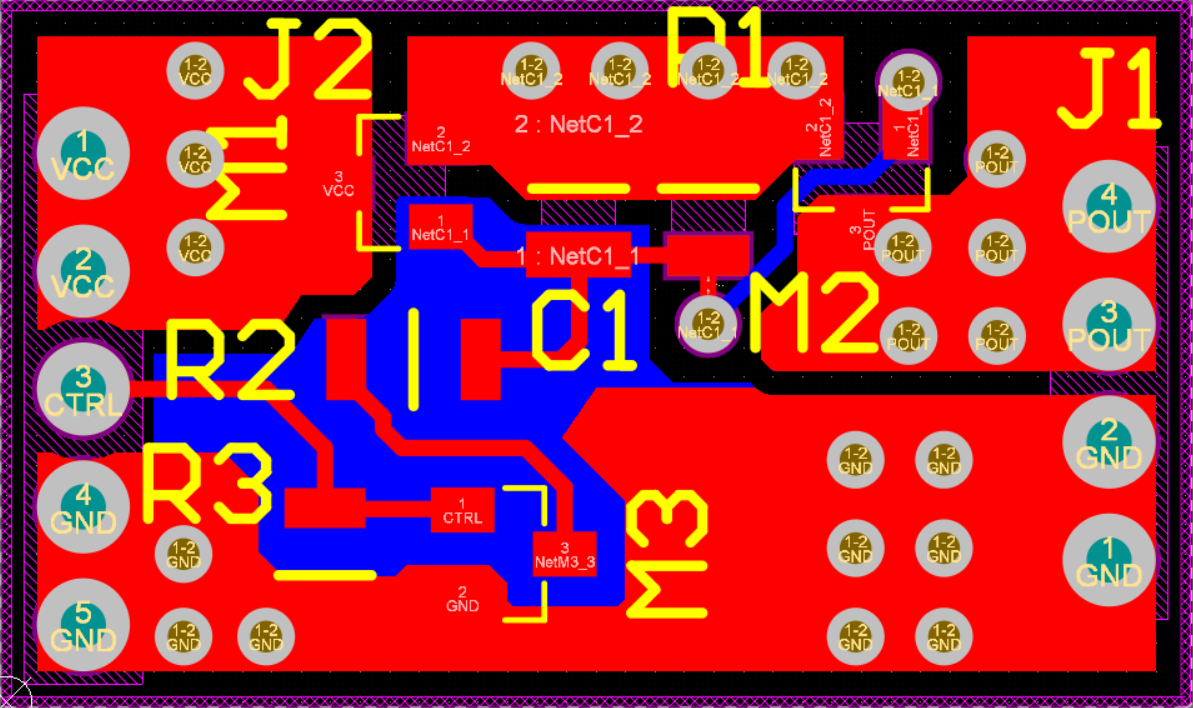
\includegraphics[scale=0.2]{imagenes/power_switch_test_top.png}
            \caption{Capa superior}
        \end{subfigure}
        \begin{subfigure}{0.45\textwidth}
            \centering
            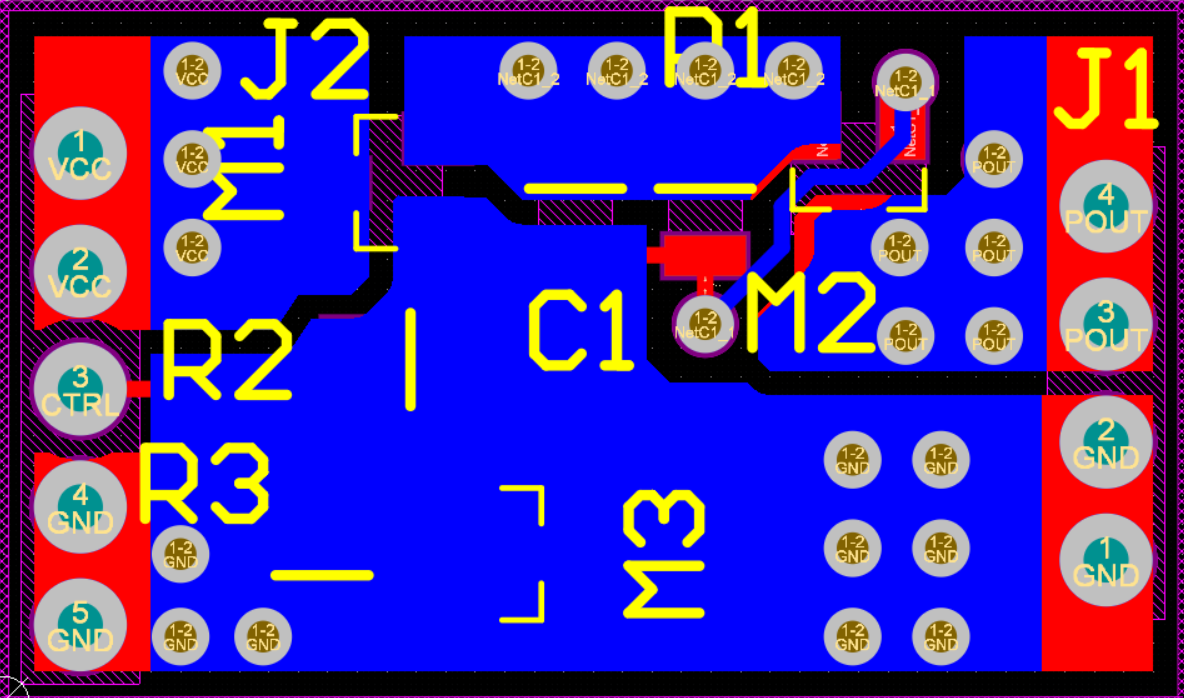
\includegraphics[scale=0.2]{imagenes/power_switch_test_bottom.png}
            \caption{Capa inferior}
        \end{subfigure}
        \vfill
        \begin{subfigure}{0.45\textwidth}
            \centering
            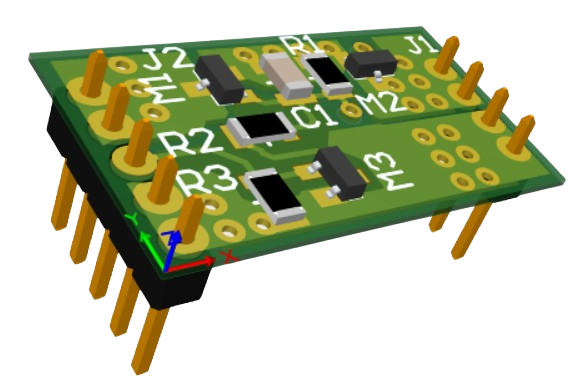
\includegraphics[scale=0.3]{imagenes/power_switch_test_3D.png}
            \caption{Vista 3D} 
        \end{subfigure}
        \begin{subfigure}{0.45\textwidth}
            \centering
            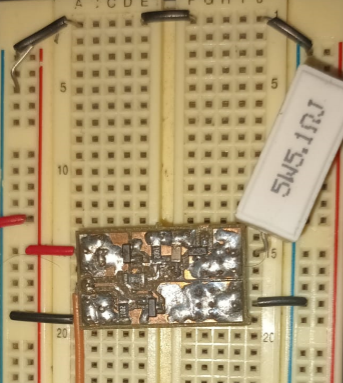
\includegraphics[scale=0.4]{imagenes/power_switch_test_asm.png}
            \caption{PCB ensamblada}
        \end{subfigure}

        \caption{Placa de pruebas del conmutador de potencia}
        \label{fig:power_switch_test}
    \end{figure}

        Al momento de realizar las pruebas el diseño del conmutador de potencia
        tuvo el comportamiento esperado, evitando el paso de corriente cuando
        el transistor MOSFET M3 no se encontraba en conducción, y permitiendo
        el paso de corriente cuando el transistor MOSFET M3 se encontraba en
        conducción. Adicionalmente se comprobó que la caída de tensión en el
        conmutador de potencia era de $0.12\Omega$ cuando se encontraba conduciendo
        una corriente de $3\text{A}$, y este no presentaba un aumento de temperatura
        significativo. En la figura \ref{fig:charger_anexo_mux} en el anexo \ref{sec:anexo_esquematico}
        se muestra el diseño final de los multiplexores de potencia.

        El diseño de este conmutador de potencia se encuentra dentro de los archivos
        adjuntos dentro de la carpeta nombrada como PCB\_Design dentro del proyecto
        de Altium nombrado como Pmos\_switch. 



    

    

    \section{Controlador}

    Para la gestión de los multiplexores de potencia y el control del convertidor
    reductor se diseñó un controlador basado en el microcontrolador ATmega328p.
    El cual tiene las siguientes funciones:

    \begin{itemize}
        \item Controlar el voltaje y corriente de salida del convertidor reductor
        \item Controlar que batería se está cargando mediante un multiplexor de potencia
        \item Controlar el multiplexor de potencia para seleccionar la batería
        que proporcionará la alimentación al agente robótico.
        \item Permitir la comunicación con la estación de carga mediante comunicación
        UART.
        \item  Permitir la comunicación con el adaptador wifi mediante comunicación
        I2C.
        \item índicar de forma visual el estado de carga de las baterías mediante
        2 LEDs.
    \end{itemize}

    
    \section{Placa de expansión para el agente robótico}

Luego de haber probado todos los sistemas en conjunto se procedió a diseñar
una placa de expansión para el agente robótico Pololu 3Pi+ que permita
la conexión de todos los sistemas diseñados. Para permitir la conexión
 entre ambas placas se utilizaron conectores 
macho ubicados según los planos proporcionados por la 
empresa Pololu \cite{noauthor_pololu_nodate}.
Los pines utilizados para la comunicación o transmisión de potencia entre
ambas placas son los siguientes:

\begin{itemize}
    \item GND: Todos los pines etiquetados como GND en la placa de control
    del agente robótico son conectados con la tierra de la placa de expansión.
    \item VBAT: Este pin es utilizado para realizar la carga de las baterías
    NiMH presentes en el agente robótico.
    \item VSW: Este pin es utilizado para alimentar la placa de 
    control del agente robótico, al momento de que la batería NiMH 
    se encuentre descargada.

\end{itemize}

Debido a la alta cantidad de componentes que se encuentran en la placa de expansión
se decidió utilizar una placa de 4 capas, con el fin de facilitar el enrutamiento
de las señales de potencia y de comunicación entre los distintos componentes. 
La placa de expansión diseñada se muestra en la figura \ref{fig:expansion_board}.

\begin{figure}[H]
    \centering
    \begin{subfigure}{0.45\textwidth}
        \centering
        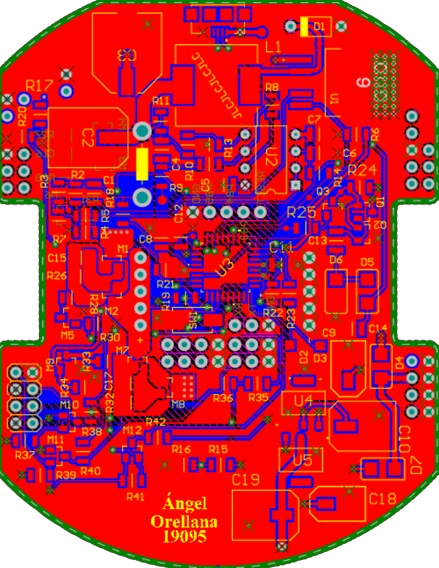
\includegraphics[scale=0.3]{imagenes/system_top.png}
        \caption{Capa superior}
    \end{subfigure}
    \begin{subfigure}{0.45\textwidth}
        \centering
        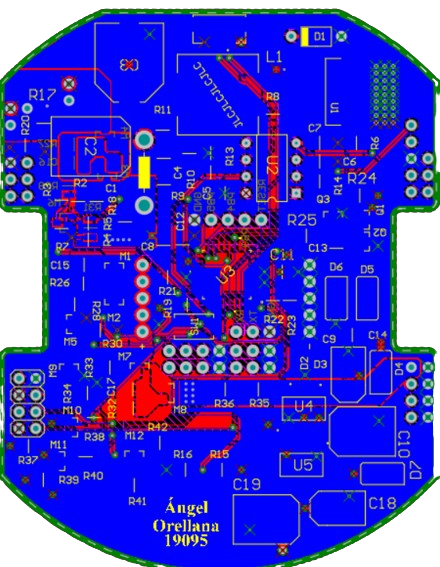
\includegraphics[scale=0.3]{imagenes/system_bottom.png}
        \caption{Capa inferior}
    \end{subfigure}
    \vfill
    \begin{subfigure}{0.45\textwidth}
        \centering
        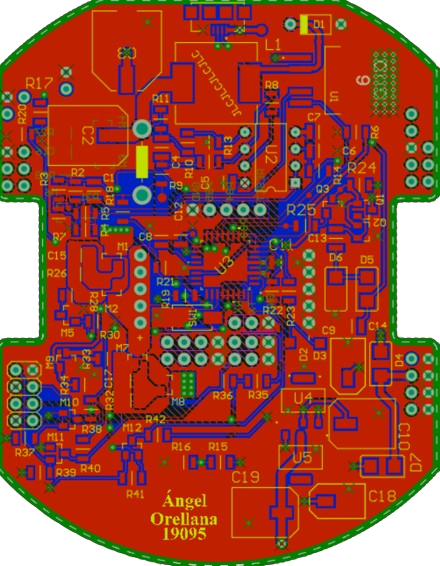
\includegraphics[scale=0.3]{imagenes/system_gnd.png}
        \caption{Plano de tierra de la placa de expansión} 
    \end{subfigure}
    \begin{subfigure}{0.45\textwidth}
        \centering
        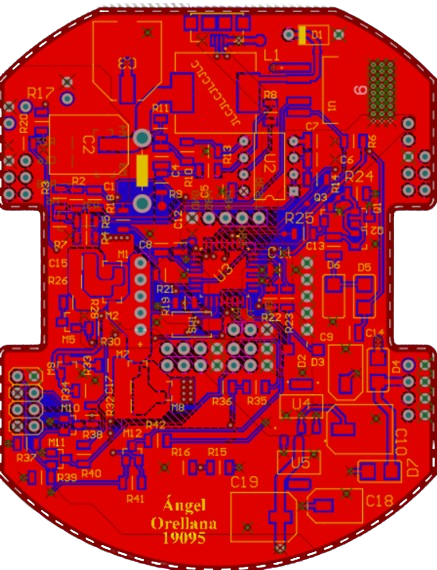
\includegraphics[scale=0.3]{imagenes/system_pwr.png}
        \caption{Plano de potencia de la placa de expansión}
    \end{subfigure}

    \caption{Placa de expansión para el agente robótico}
    \label{fig:expansion_board}
\end{figure}

Para comprobar que la placa de expansión diseñada se alinea correctamente
con la placa de control del agente robótico se realizó descargó el modelo
3D de la placa de control del agente robótico desde la página web de Pololu
\cite{noauthor_pololu_nodate}, y se realizó el ensamblaje de ambas placas
en el software Altium Designer, el resultado del ensamblaje se muestra en
la figura \ref{fig:expansion_board_assembly}.

\begin{figure}[H]
    \centering
    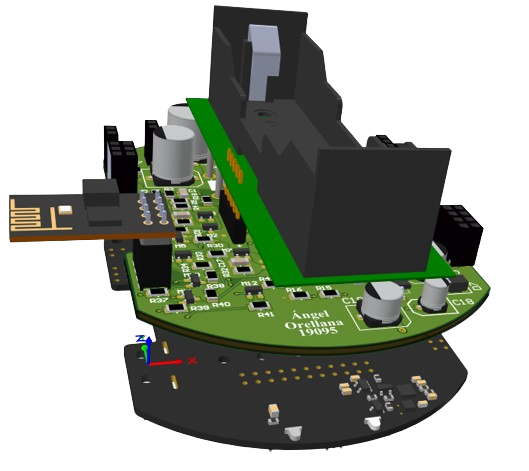
\includegraphics[scale=0.5]{imagenes/system_assembly.png}
    \caption{Ensamblaje de la placa de expansión con la placa de control del agente robótico}
    \label{fig:expansion_board_assembly}
\end{figure}

\subsection{Pruebas de la placa de expansión}

Para comprobar el correcto funcionamiento de la placa de expansión diseñada,
principalmente se realizaron pruebas de comunicación entre la placa de expansión
y la placa de control del agente robótico, y pruebas de alimentación de la placa
de control del agente robótico. Para comprobar que no existiera una interrupción
en la alimentación de la placa de control del agente robótico al momento de 
realizar el cambio de batería se utilizó el programa mostrado en el apéndice
\ref{sec:codigo_prueba_expansion}, el cual corresponde al proyecto de MPLAB
nombrado como Pololu\_on\_test.X, dentro de la carpeta nombrada como Charge\_system\_firmware.

En la figura \ref{fig:expansion_board_test} se muestra la placa de expansión
conectada a la placa de control del agente robótico.

\begin{figure}[H]
    \centering
    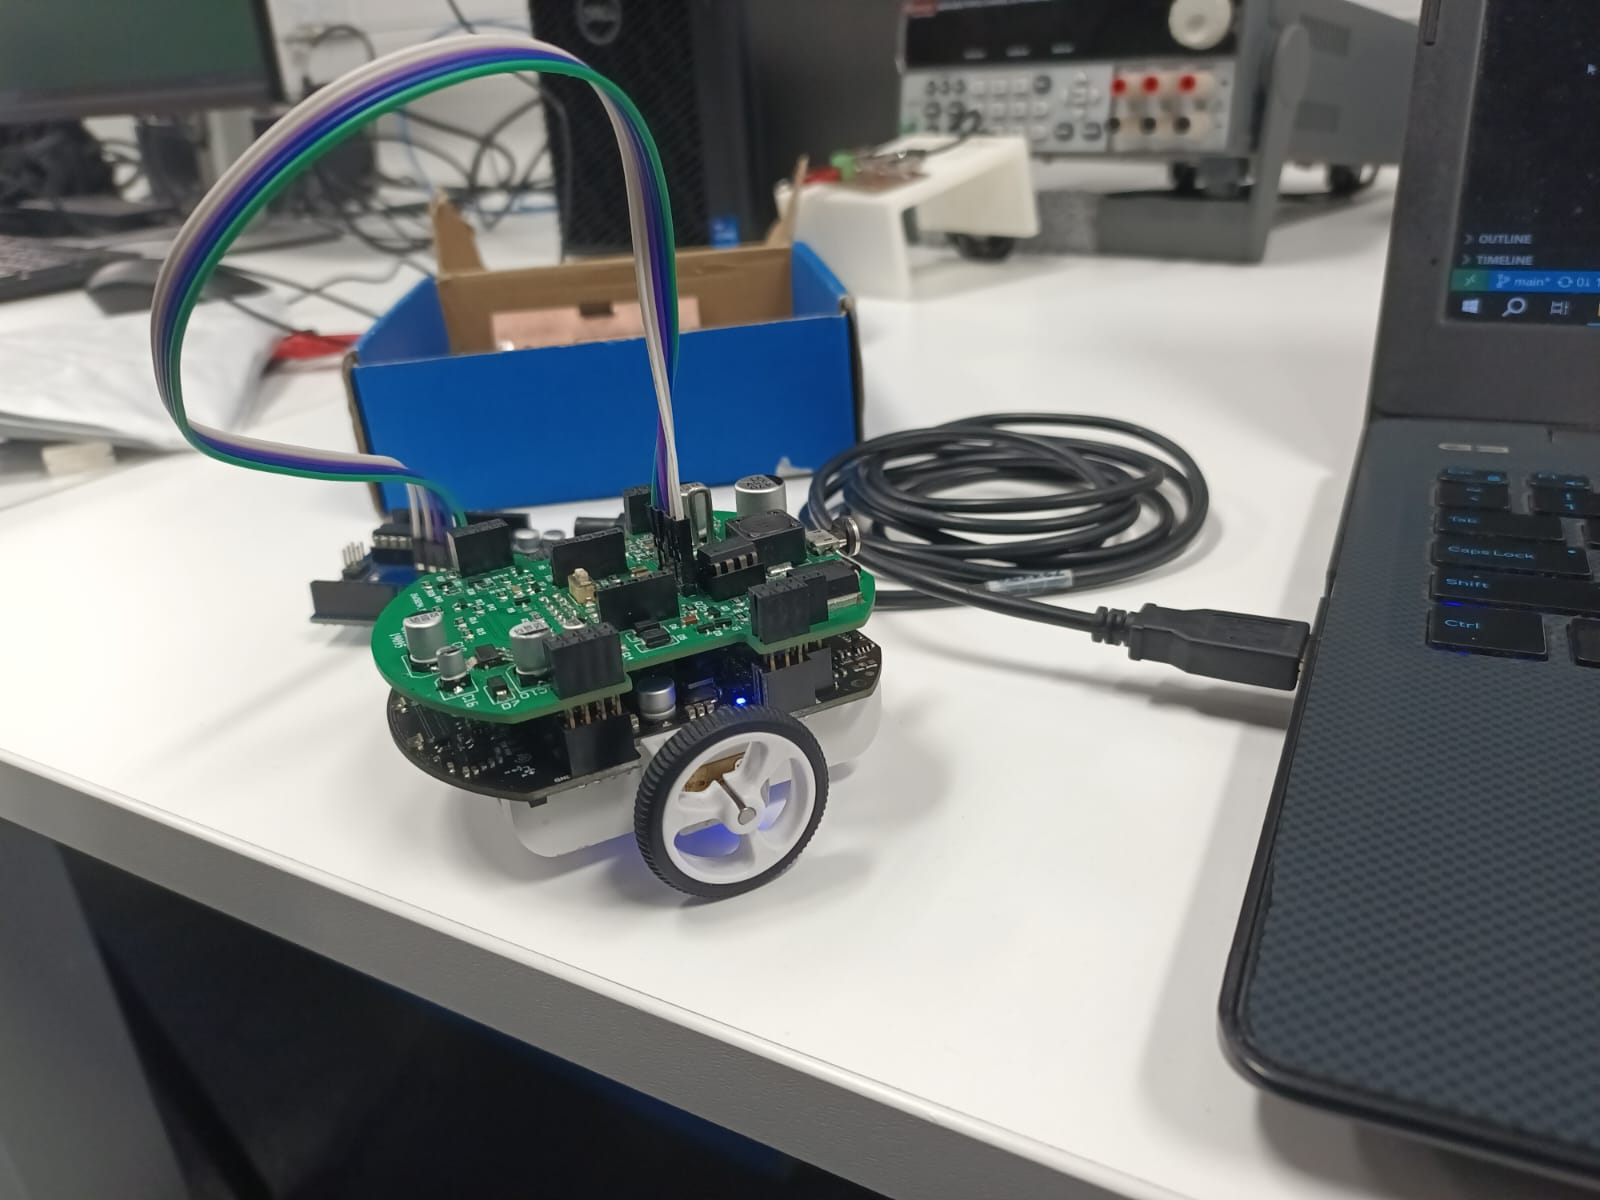
\includegraphics[scale=0.2]{imagenes/system_test.jpg}
    \caption{Prueba de la placa de expansión}
    \label{fig:expansion_board_test}
\end{figure}

El programa final de la placa de expansión se muestra en el apéndice \ref{sec:codigo_expansion},
el cual corresponde al proyecto de MPLAB nombrado como Pololu\_on.X, dentro de la carpeta





    
        

\chapter{Estación de carga}

La estación de carga está compuesta por 2 partes, la primera es un circuito impreso
en el cual se encuentran los conectores USB, para la transmisión de potencia y 
datos entre la estación de carga y el sistema de carga multiquímica. La segunda
parte es una estructura impresa en 3D, la cual tiene como función principal
proveer un espacio para colocar el circuito impreso descrito anteriormente y 
los cables USB magnéticos que se utilizarán para realizar la conexión entre
la estación de carga y el sistema de carga multiquímica.


\section{Circuito impreso}

El circuito impreso tiene 4 componentes principales que se listan a continuación:

\begin{itemize}
    \item Conectores USB tipo A hembra
    \item Cables USB para transmisión de potencia
    \item \textit{Headers} macho para comunicación serial
    \item Bornera de 2 pines para alimentación de la estación de carga
\end{itemize}
El circuito impreso diseñado se muestra en la figura \ref{fig:pcb_estacion_carga}.

\begin{figure}[H]
    \centering
    \begin{subfigure}{0.9\linewidth}
        \centering
        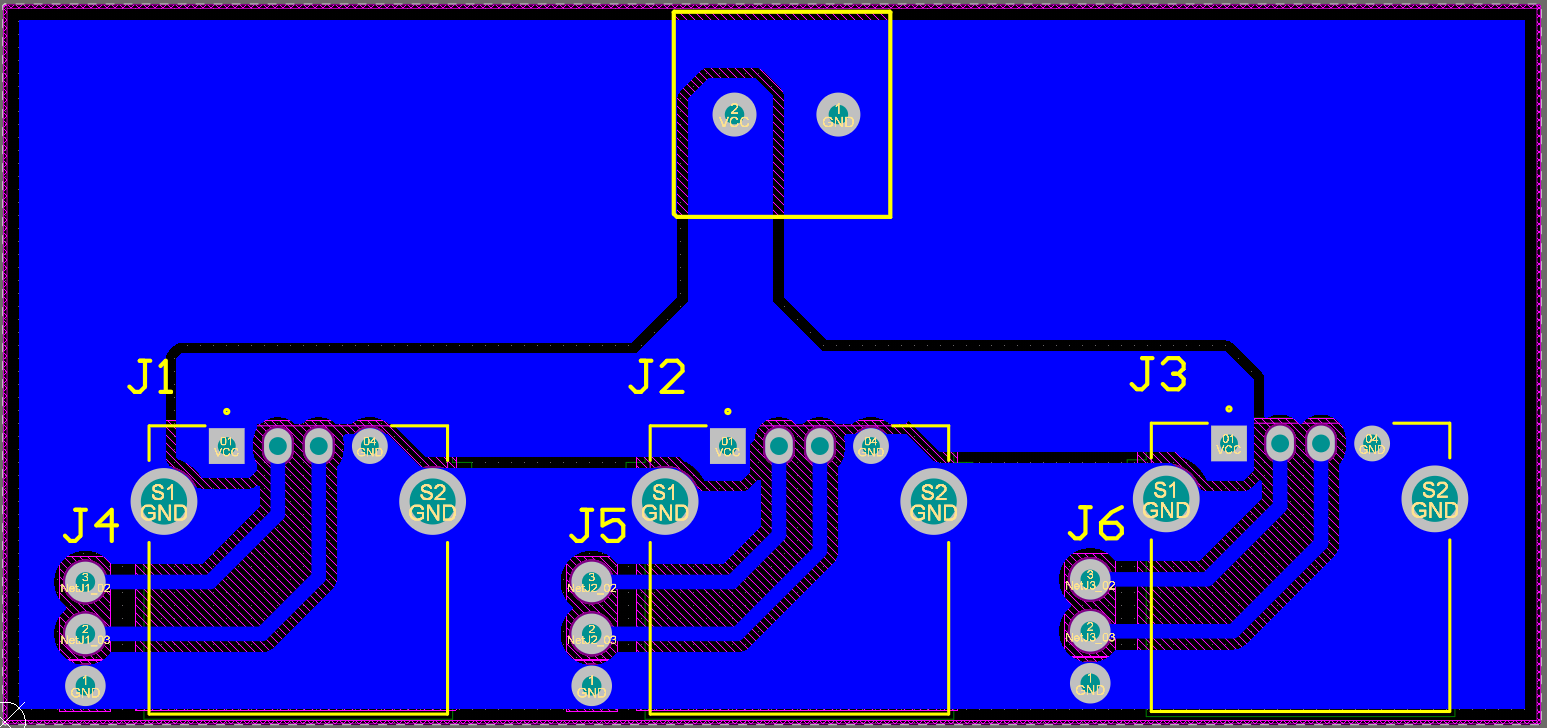
\includegraphics[scale=0.25]{imagenes/bottom_charging.png}
        \caption{Capa inferior}
    \end{subfigure}
    \vfill
    \begin{subfigure}{0.9\linewidth}
        \centering
        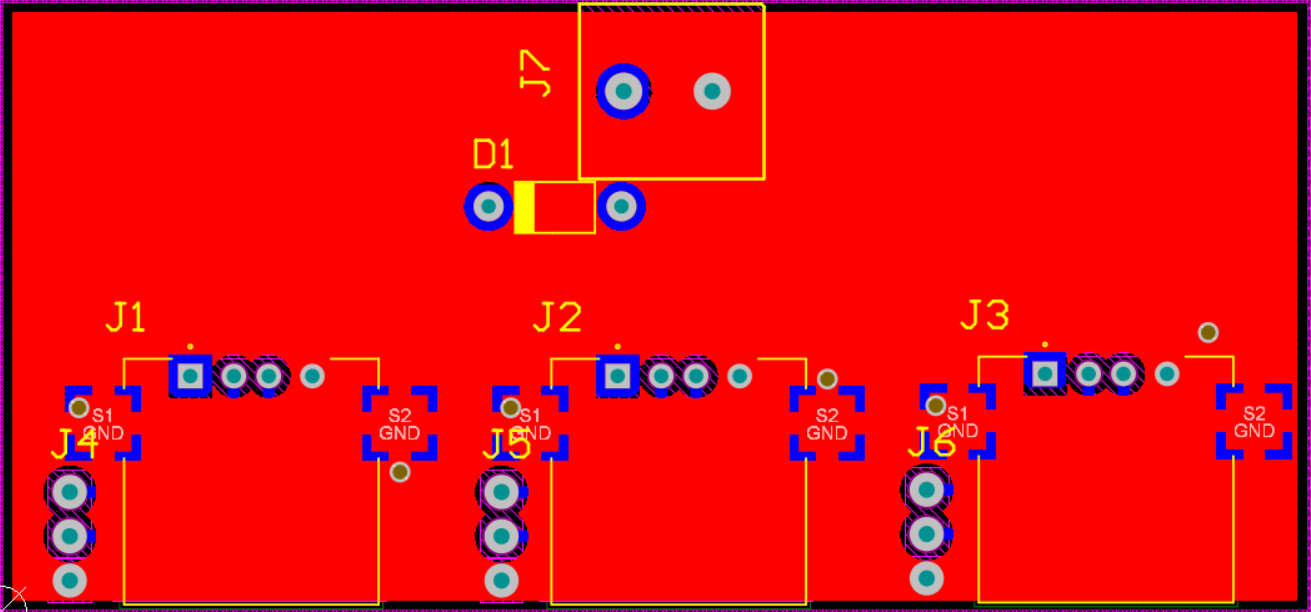
\includegraphics[scale=0.25]{imagenes/top_charging.png}
        \caption{Capa superior}
    \end{subfigure}
    \vfill
    \begin{subfigure}{0.9\linewidth}
        \centering
        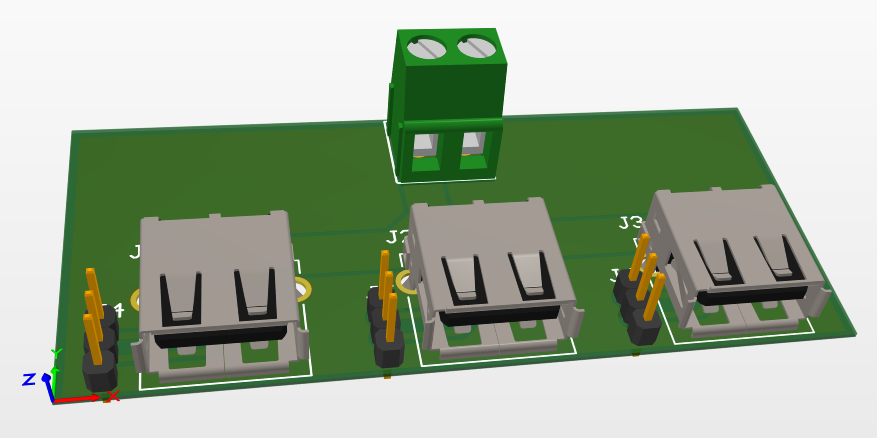
\includegraphics[scale=0.45]{imagenes/3d_charging.png}
        \caption{Vista 3D}
    \end{subfigure}
    \caption{Diseño del PCB para la estación de carga}
    \label{fig:pcb_estacion_carga}
\end{figure}

Para sujetar el circuito impreso en el borde de la arena de Robotat se diseñó 
una estructura impresa en 3D, la cual se muestra en la figura \ref{fig:3d_estacion_carga}.
La estructura impresa en 3D colocada en el borde arena de Robotat se muestra en la
 figura \ref{fig:estacion_carga_ensamblaje}.

\begin{figure}
    \centering
    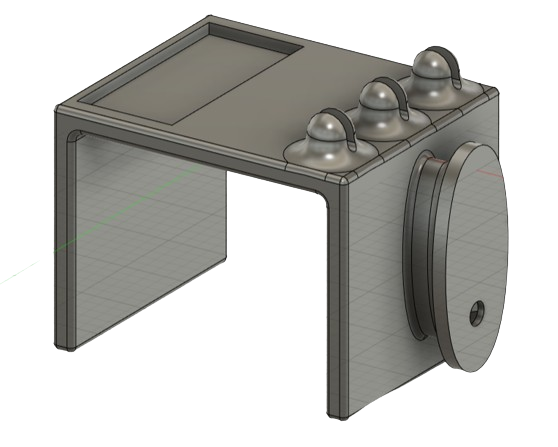
\includegraphics[scale=0.3]{imagenes/estacion_de_carga.png}
    \caption{Diseño de la estructura impresa en 3D para la estación de carga}
    \label{fig:3d_estacion_carga}
\end{figure}

\begin{figure}[H]
    \centering
    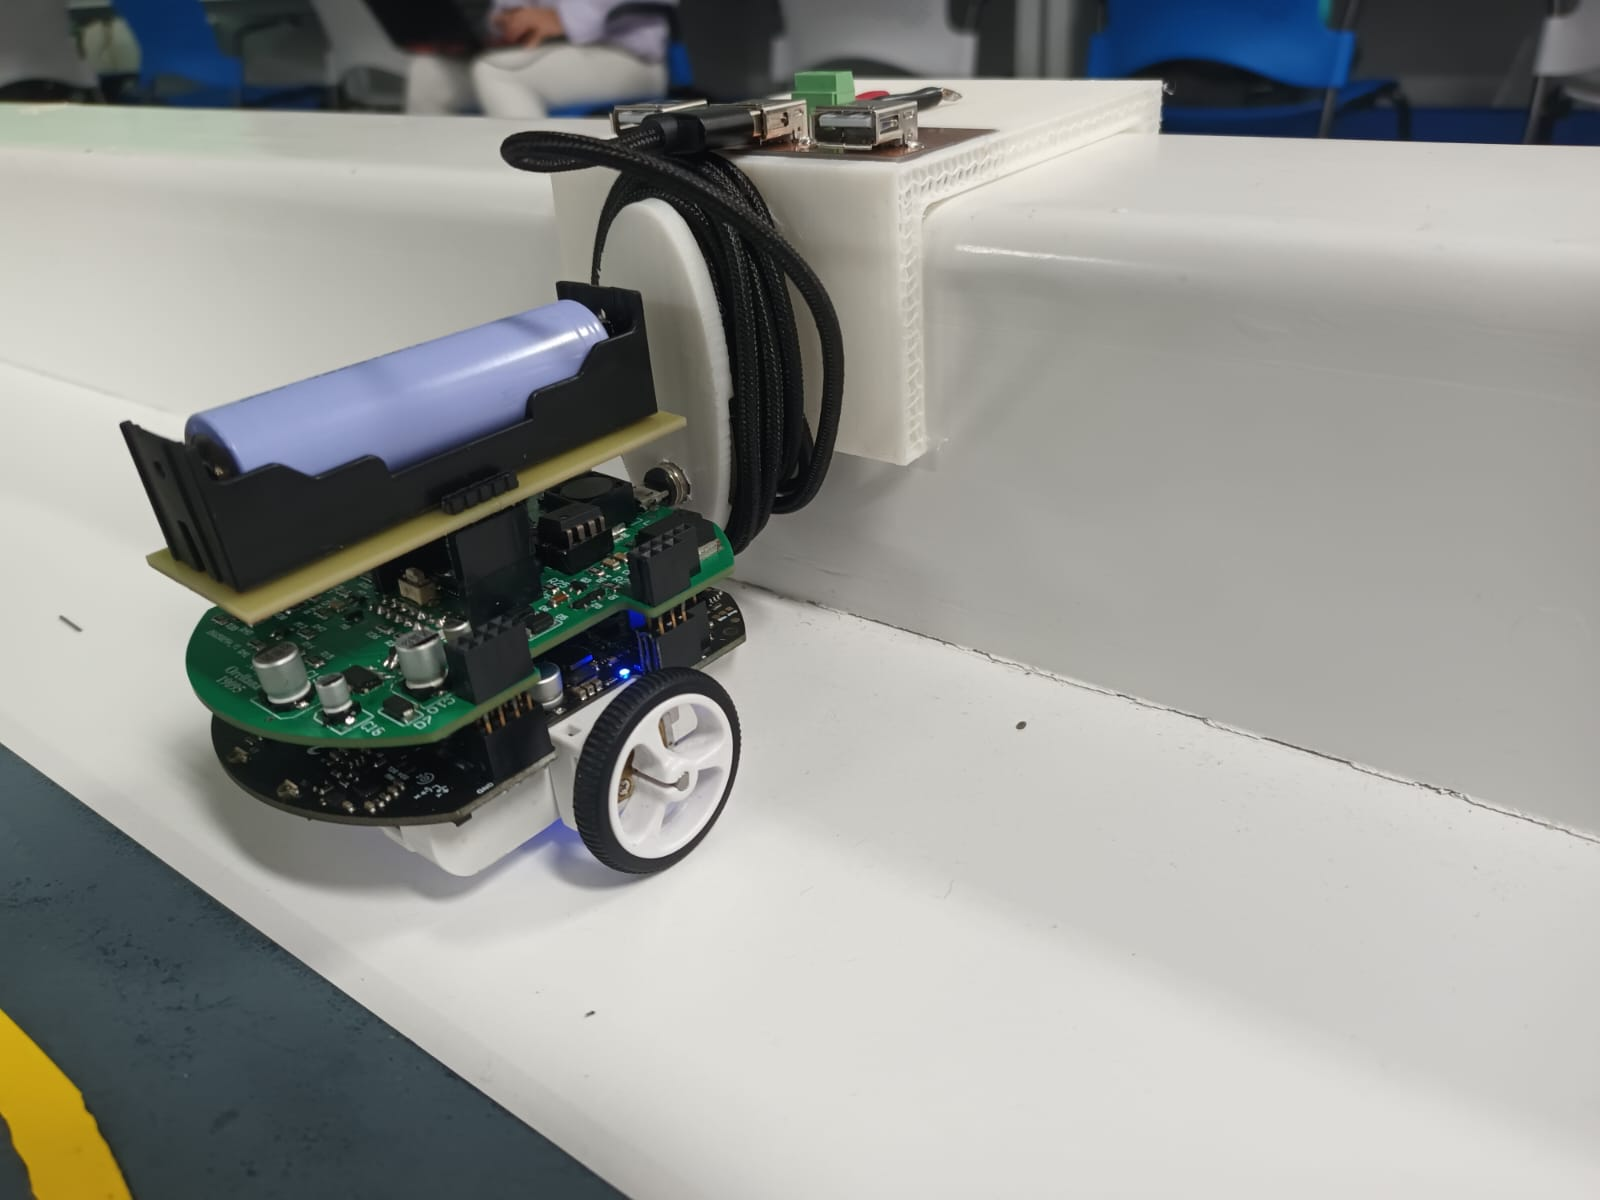
\includegraphics[scale=0.15]{imagenes/estacion_carga_ensamblaje.jpg}
    \caption{Ensamblaje de la estación de carga}
    \label{fig:estacion_carga_ensamblaje}
\end{figure}

Debido al tipo de cable empleado no es posible realizar comunicación UART entre
la estación de carga y el sistema de carga multiquímica, debido a que los cables
USB magnéticos no cuentan con los pines necesarios para realizar la comunicación, 
sin embargo, es posible realizar la comunicación UART con el sistema de carga
multiquímica a través de pines macho que se encuentran en la placa de expansión
del sistema de carga multiquímica. 